%=================================================================
% MIMO vs. Decentralized Droop-Share / Drive Control — INTERNAL LAB REPORT
%
% NOT FOR PUBLICATION. Internal lab circulation only.
%=================================================================
\documentclass[energies,article,submit,pdftex,oneauthor]{Definitions/mdpi}

% ---- Extra packages (mdpi.cls already loads amsmath, amssymb, graphicx,
%      booktabs, float, tabularx, xcolor, draftwatermark) ----
\usepackage{siunitx}
\usepackage{tabularx}
\newcolumntype{C}{>{\centering\arraybackslash}X} % centered X column for comparison tables

% MDPI internal commands - do not modify
\firstpage{1}
\makeatletter
\setcounter{page}{\@firstpage}
\makeatother
\pubvolume{1}
\issuenum{1}
\articlenumber{0}
\pubyear{2026}
\copyrightyear{2026}
\datereceived{ }   % TODO: internal report — no journal dates
\daterevised{ }
\dateaccepted{ }
\datepublished{ }
\hreflink{https://doi.org/}   % TODO: internal report — no DOI

\Title{MIMO versus Decentralized Control of the Coupled Droop-Share and
Drive Loops on the SC001 Balancer Board: An Internal Comparison}
\TitleCitation{MIMO versus Decentralized Control of the Coupled Droop-Share and Drive Loops: An Internal Comparison}

\newcommand{\orcidauthorA}{0009-0009-3531-2294}

\Author{Ricky Tan $^{1}$\orcidA{}}
\AuthorNames{Ricky Tan}
\isAPAStyle{%
       \AuthorCitation{Tan, R.}
         }{%
        \isChicagoStyle{%
        \AuthorCitation{Tan, Ricky.}
        }{
        \AuthorCitation{Tan, R.}
        }
}
\address[1]{%
Department of Mechanical \& Aerospace Engineering, University of California, Davis, CA 95616,
USA; rstan@ucdavis.edu}
\corres{\hangafter=1 \hangindent=1.05em \hspace{-0.82em}Correspondence: rstan@ucdavis.edu}

\abstract{The SC001 scale car carries two independently designed robust loops: an
$H_\infty$/Youla-H current-share controller that commands a droop ratio between a fuel cell and
a battery, and a vehicle-speed drive controller. Both were designed single-input single-output,
on the assumption that the two loops do not interact. This report tests that assumption. We
build a $2\times2$ small-signal design plant in which the drive channel disturbs the share
channel through the bus current it draws, validate it against an independent 15-state
converter-level model, synthesize a centralized $2\times2$ $H_\infty$ controller with a matrix
generalization of the Youla-H DC-correction recipe that makes $T(0)=I$ structural, and compare
it head-to-head against the decentralized pair on the same coupled plant, the same corner
families and the same simulations. The coupling is one-directional, so the relative gain array
is provably uninformative; the informative measure is the directional ratio
$|G_{s,12}|/|G_{s,11}|$ on the error- and actuator-normalized plant, which is $1.57$ at the
nominal $\SI{2}{\ampere}$ load and $25.1$ at $\SI{0.5}{\ampere}$.
The comparison gives three different answers on the three primary metrics:
the centralized controller outperforms the decentralized pair on worst-corner sensitivity by
$27\,\%$, ties on regen bus excursion, and is superior or inferior on
drive-transient share excursion depending on the sign of an uncalibrated source-voltage mismatch
$\Delta V_0$. Decentralized control is stable at all $4992$ feasible corners, retains a
$2.3\times$ drive-cycle tracking advantage, and does not depend on that sign. We conclude that
decentralization is justified on its merits, and that measuring $\Delta V_0$ on
the bench is the single highest-value action for narrowing the remaining uncertainty.
Methodologically, the actuator limit functions as a design node: it
sets the input scaling, hence the effective control-effort penalty, and hence the achievable
robustness.}

\keyword{$H_\infty$ control; Youla parameterization; MIMO control; droop control; power
sharing; decentralized control; hybrid vehicle; DC bus}

%%%%%%%%%%%%%%%%%%%%%%%%%%%%%%%%%%%%%%%%%%
\begin{document}

% NOTE: the class loads an older draftwatermark that has no \SetWatermarkText;
% the internal marking is the notice line below plus the title/abstract wording.
\begin{center}
\itshape Internal lab report --- not for external distribution or publication. Numbers are
generated artefacts of the \textup{\texttt{controller\_design\_MIMO}} pipeline; nothing here
is bench-calibrated.
\end{center}

%%%%%%%%%%%%%%%%%%%%%%%%%%%%%%%%%%%%%%%%%%
\section{Introduction}
\label{sec:introduction}

The SC001 scale car's DC balancer board routes power from a fuel cell and a battery onto a
shared bus through two off-the-shelf boost regulators whose output resistance is made
electronically programmable by injecting a shunt-derived, multiplying-DAC-scaled signal into
each converter's feedback node. The resulting \emph{droop ratio} $r$ is the actuator of a
current-share loop whose output is the share fraction $\alpha = I_{FC}/(I_{FC}+I_{BT})$, closed
by a robust $H_\infty$/Youla-H controller synthesized against a 60-corner uncertain plant family
and documented separately \citep{internal:droop}. The vehicle's speed is regulated by a second
loop that commands motor current through a VESC over UART, following the drive-controller recipe
of \citep{tan2025scaling} with the post-synthesis DC correction of \citep{tan2025youlah}.

Both loops were designed single-input single-output, each on its own plant, each validated only
against its own uncertainty family. That separation was assumed without derivation: the two
loops share a bus, and every ampere the motor draws is an ampere the two sources must split.
This report tests whether the decentralized design is genuinely
justified or merely convenient. Three metrics decide it --- worst-corner $\|S\|_\infty$,
drive-transient share excursion, and regen-event bus excursion \citep{internal:droop}.

Two safeguards keep the comparison from being decided by its own construction. \emph{Both}
controllers are closed against the same coupled $2\times2$ plant with the same assembly routine,
corner sets and simulator, so the decentralized pair is never evaluated on a diagonal plant; and
the amplitude of every excitation is stated, with every case in which the
$\pm\SI{20}{\ampere}$ motor-current clamp is active flagged.

\subsection{Contributions}
\begin{itemize}
\item A $2\times2$ small-signal design plant for the coupled share/drive problem
      (Section~\ref{sec:model}), in which the drive-to-share coupling is \emph{derived} from the
      static share law instead of asserted, and is reproduced endogenously to $0.032\,\%$ by an
      independent 15-state converter-level model (Appendix~\ref{app:fullorder}).
\item The observation that the plant is structurally upper-triangular, so the relative gain array
      is the identity at every frequency and every corner and carries no information; the
      informative measure is the directional ratio $|G_{s,12}|/|G_{s,11}|$.
\item A matrix generalization of the scalar Youla gain-tuning recipe that enforces $T(0)=I$ on a
      MIMO loop by a constant right multiplier on the Youla parameter, made \emph{structural} by
      an exact rank-2 integrator split (Section~\ref{sec:youlah}).
\item A head-to-head comparison on identical terms (Section~\ref{sec:comparison}), whose result
      is that the three primary metrics give three different answers, backed by an independent
      MATLAB cross-validation of the whole chain (Appendix~\ref{app:matlab}).
\end{itemize}

%%%%%%%%%%%%%%%%%%%%%%%%%%%%%%%%%%%%%%%%%%
\section{The Coupled $2\times2$ Plant}
\label{sec:model}

\subsection{Notation}
\label{sec:notation}

The share literature, the powertrain-Youla papers and the firmware reuse the same letters for
different quantities. Table~\ref{tab:notation} is binding here; the three collisions that
matter in practice are $r$ (droop ratio, never tire radius --- that is $r_t$), $\alpha$ (current
share, never an acceleration) and $K$ (share-plant DC gain, never a controller gain or motor
$K_V$).

\begin{table}[H]
\caption{Notation. Small-signal deviations carry a leading $\Delta$.}
\label{tab:notation}
\begin{tabularx}{\textwidth}{llX}
\toprule
\textbf{Symbol} & \textbf{Units} & \textbf{Meaning (and what it is \emph{not})} \\
\midrule
$r$ & --- & Droop ratio command, $r\in[0.15,0.85]$. \emph{Not} tire radius. \\
$r_t$ & \si{\meter} & Tire radius, \num{0.033}. \\
$\alpha$ & --- & Current share $I_{FC}/(I_{FC}+I_{BT})$; the share-loop output. \emph{Never} an acceleration. \\
$k_d$ & \si{\ohm} & Droop scale, \num{0.30} (firmware \texttt{K\_DROOP}). \\
$R_{e,max}$ & \si{\ohm} & Full-scale programmable output resistance, \num{2.014} (as-built). \\
$\Delta V_0$ & \si{\volt} & No-load source-voltage mismatch, FC vs.\ BT; $\pm\num{0.4}$ budget, sign unknown. \\
$I_{tot}$ & \si{\ampere} & Total bus current out of the two sources. \\
$K$ & --- & Share-plant DC gain $\partial\alpha/\partial r$ at the operating point. \\
$K_v$ & --- & Drive-channel structural gain uncertainty multiplier, $\in\{0.5,1,2\}$. \\
$k_t$, $\varphi$, $b_{\!e\!f\!f}$ & --- & Motor torque constant, drive ratio \num{9.49}:1, wheel-referred damping. \\
$G$, $G_s$ & --- & Design plant; $G_s = D_e^{-1} G D_u$ its scaled form. \\
$S$, $T$, $Y$; $W_p$, $W_{\Delta}$, $W_u$ & --- & Sensitivity, complementary sensitivity, Youla transfer function ($2\times2$), and the $H_\infty$ cost weights on each ($W_{\Delta}$, also written $W_3$, is the robustness weight on $T$). \\
$M_{YH}$, $\gamma$ & --- & MIMO Youla-H DC correction matrix $[G_s(0)Y_H(0)]^{-1}$; $H_\infty$ level. \\
$M_2$ & --- & $M_2 = 1/\|S\|_\infty$, the $M_2$ stability margin (Def.~4.2 of \citep{assadian2020neoclassical}). \\
$P_c$, $P_f$ & --- & DGKF control and filter Riccati solutions. \emph{Not} $X$/$Y$ --- $Y$ is the Youla transfer function. \\
\bottomrule
\end{tabularx}
\end{table}

The symbols $S$, $T$, $Y$, $L$, $G_p$ and $G_c$ follow \citep{assadian2020neoclassical}
(pp.~xxxi--xxxii, 88--91, 393--395), including that body's definition of $Y = G_c S$ as the
\emph{Youla transfer function (matrix)} --- which is why $Y$ is not available here as a Riccati
solution symbol.

The plant inputs and outputs are
\begin{equation}\label{eq:io}
u = \begin{bmatrix} \Delta r \\ \Delta i_{cmd} \end{bmatrix}, \qquad
y = \begin{bmatrix} \Delta \alpha \\ \Delta v \end{bmatrix},
\end{equation}
with actuator limits $r\in[0.15,0.85]$ and $|i_{cmd}|\le\SI{20}{\ampere}$. Native rates are
\SI{1}{\kilo\hertz} for the share loop and \SI{500}{\hertz} for the motor loop, the latter set by
the VESC UART frame floor of roughly \SI{781}{\micro\second}.

\subsubsection{The actuator limit}
The motor-current clamp is a \emph{motor-side} limit, but the constraint it must respect lives on
the \emph{bus}: the two converters can supply roughly \SIrange{67}{87}{\watt} between them. The
two are related by the bus-current conversion $A_i \approx
\SI{0.243}{\ampere\per\ampere}$ of \eqref{eq:Ibus}, so a $\pm\SI{20}{\ampere}$ motor-side clamp is
$\approx\SI{4.9}{\ampere}$ bus-side at cruise, $\approx\SI{77}{\watt}$ at
$V_{bus0} = \SI{15.9}{\volt}$ --- inside that budget, and close enough to it that the motor clamp
and the converter power budget bind \emph{together} by construction. The bus-power limit is
therefore not carried as a separate modelled constraint: at the cruise operating point it is
approximately equivalent to the motor clamp, and away from that point it is the motor clamp that
is quoted. A clamped case is therefore one in which the powertrain as a whole is at its limit, not
one in which an arbitrarily chosen number is.

\subsection{Share channel}

The droop hardware realizes a commanded output resistance $R_e(g) = R_{e,max}\,g$ per channel;
mapping the ratio as $R_F = k_d/r$, $R_B = k_d/(1-r)$ gives $R_F \parallel R_B = k_d$
independently of $r$, so the bus droop is decoupled from the split. Solving the two-Th\'evenin
circuit yields the exact static share law \citep{internal:droop}
\begin{equation}\label{eq:share}
\alpha(r, I_{tot}) \;=\; r \;+\; \frac{\Delta V_0\, r(1-r)}{k_d\, I_{tot}},
\end{equation}
whose $r$-derivative is the share-plant DC gain
\begin{equation}\label{eq:K}
K \;=\; \frac{\partial\alpha}{\partial r} \;=\; 1 + \frac{\Delta V_0 (1-2r_0)}{k_d\, I_{tot0}} .
\end{equation}
The share channel of the design plant is then the SISO share plant of \citep{internal:droop}
unchanged,
\begin{equation}\label{eq:G11}
G_{11}(s) = K\cdot \mathrm{Pad\acute{e}}_2\!\left(e^{-T_d s}\right)\cdot
\frac{1}{\tau_r s + 1}\cdot\frac{1}{\tau_f s + 1},
\end{equation}
with $T_d = \SI{1}{\milli\second}$ nominal loop delay, $\tau_r = \SI{100}{\micro\second}$, and
$\tau_f = \SI{0.8}{\milli\second}$ the firmware's \SI{200}{\hertz} share-measurement prefilter;
it reproduces the SISO plant to $8.0\times10^{-16}$ relative over all operating points and five
parameter corners.

\subsection{Drive channel}

The drive channel is a VESC transport delay and current-loop lag feeding a force constant and a
first-order longitudinal mode:
\begin{equation}\label{eq:G22}
G_{22}(s):\quad \Delta i_{cmd} \to \mathrm{Pad\acute{e}}_2\!\left(e^{-T_{d,v} s}\right)
\to \frac{1}{\tau_v s + 1} \to \frac{k_t \eta_{dt}\varphi}{r_t}\ [\si{\newton\per\ampere}]
\to \frac{1}{m_{\!e\!f\!f} s + b_{\!e\!f\!f}} \to K_{enc}K_v ,
\end{equation}
with DC gain $G_{22}(0) = K_{enc}K_v k_t \eta_{dt}\varphi/(r_t b_{\!e\!f\!f}) =
\SI{3.7085}{\meter\per\second\per\ampere}$ and a mechanical pole at
$-b_{\!e\!f\!f}/m_{\!e\!f\!f} = \SI{-0.1219}{\radian\per\second}$ --- a near-integrator, an
\SI{8}{\second} time constant. This recovers the powertrain form of \citep{tan2025scaling}
exactly when $b$ is written shaft-referred; here it is written wheel-referred, with the motor's
spinning loss reflected in through $b_{motor}(\varphi/r_t)^2$.

Two features of $b_{\!e\!f\!f}$ are counter-intuitive. At the nominal operating point aero
contributes \SI{0.0245}{\newton\second\per\meter} and the motor's own free-run loss
\SI{0.3352}{}, so the motor dominates the small-signal damping by $14\times$. And rolling
resistance is Coulomb: it sets the operating-point torque (hence the coupling gains below) but
its derivative with respect to $v$ is zero away from standstill, so it must \emph{not} appear in
$b_{\!e\!f\!f}$. The gain uncertainty $K_v\in\{0.5,1,2\}$ is structural in origin: the
encoder sits downstream of the \num{9.49}:1 reduction \emph{and} the limited-slip differentials,
so there is no fixed rotor-to-ground-speed mapping, and $k_t$ is uncalibrated because no motor
has been selected.

\subsection{Coupling}

$G_{21}=0$ is a modelling \emph{result}: the droop ratio reaches no state that
feeds the speed output in either the design plant or the truth model, because the VESC runs a
current loop: at fixed $i_{cmd}$ the delivered torque is independent of $v_{bus}$ until the duty
rail. The residual this discards is measured --- $|\Delta v_{bus}/\Delta r|$ at DC is
\SI{0.2002}{\volt} per unit $r$, $0.44\,\%$ of the \SI{15.9}{\volt} bus over the full $r$ span
--- well below duty saturation throughout the envelope. It would break under deep battery
discharge with a large $i_{cmd}$, or a regen event pushing the bus into overvoltage protection;
both lie outside the linear envelope and are handled by the firmware's sequencing layer.

The live coupling is $G_{12}$, drive to share, in two stages. Linearizing motor input power
$P = (k_t\omega i_m + R_m i_m^2)/\eta_v$ about the operating point at fixed $V_{bus0}$ gives the
bus-current draw
\begin{equation}\label{eq:Ibus}
\Delta I_{bus} = A_i\,\Delta i_m + A_\omega\,\Delta\omega, \qquad
A_i = \frac{k_t\omega_0 + 2R_m i_{m0}}{\eta_v V_{bus0}}, \qquad
A_\omega = \frac{k_t i_{m0}}{\eta_v V_{bus0}} ,
\end{equation}
numerically $A_i = \SI{0.24292}{\ampere\per\ampere}$ and
$A_\omega = \SI{3.9272e-4}{\ampere\per\radian\per\second}$ at nominal. The $\Delta\omega$ term is
what makes the coupling \emph{dynamic} rather than a static feedthrough: it routes through the
vehicle mode, so the coupling inherits the near-integrator pole. Differentiating
\eqref{eq:share} with respect to total current gives the share sensitivity
\begin{equation}\label{eq:dalpha}
\frac{\partial\alpha}{\partial I_{tot}} \;=\; -\,\frac{\Delta V_0\, r_0(1-r_0)}{k_d\, I_{tot0}^2},
\end{equation}
so that $G_{12}(s) = (\partial\alpha/\partial I_{tot})\left[A_i W_v(s) + A_\omega(\varphi/r_t)
\frac{1}{m_{\mathrm{eff}}s+b_{\mathrm{eff}}} W_v(s)\right]/(\tau_f s + 1)$ with $W_v$ the VESC
path and $1/(m_{\mathrm{eff}}s+b_{\mathrm{eff}})$ the vehicle mode. At nominal
$\partial\alpha/\partial I_{tot} = \SI{-4.1667e-2}{}$ share per ampere and
$G_{12}(0) = \SI{-2.7573e-2}{}$ share per ampere of $i_{cmd}$.

Both $G_{11}$ and $G_{12}$ pass through the \emph{same} instance of the prefilter
$1/(\tau_f s+1)$, because there is exactly one such filter in firmware, downstream of the share
estimate; the plant is therefore assembled as explicit block state-space instead of a
block-diagonal composition, since duplicating the filter would add a spurious state and
misrepresent the hardware. The nominal assembly is 8 states.

\subsubsection{Sign uncertainty of the coupling}
Equation~\eqref{eq:dalpha} is \emph{exactly zero} at $\Delta V_0 = 0$ (matched sources: no
coupling) and \emph{flips sign} over the $\pm\SI{0.4}{\volt}$ budget, which is an uncalibrated
quantity. A centralized controller synthesized at one sign of $\Delta V_0$ implements a coupling
feedforward of the wrong sign at the mirror corner. Both signs are therefore mandatory in every
evaluation below.

\subsection{Why the RGA is the wrong instrument}

The design plant is upper triangular, so its relative gain array is the identity ---
$\max|\mathrm{RGA}-I| = \SI{2.23e-16}{}$ across all frequencies and all cases, including
$\Delta V_0 = \pm 0.4$. This is a property of \emph{triangularity}:
$\mathrm{RGA}(T)=I$ for any triangular $T$ no matter how large the off-diagonal entry. The RGA is
blind to one-way coupling and must not be used as the coupling metric here.

The informative measures, computed on the scaled plant, are the directional ratio
$|G_{s,12}|/|G_{s,11}|$ and the condition number
(\citep{assadian2020neoclassical} \S12.7, p.~414)\footnote{That source writes the condition
number $K(\cdot)$; this report writes $\mathrm{cond}(\cdot)$ to avoid collision with its several
$K$-symbols (Table~\ref{tab:notation}).} (Table~\ref{tab:coupling},
Figure~\ref{fig:coupling-sigma}). Both are computed on the scaled plant, so both inherit the
normalization: a ratio of unity means ``a full-authority motor command moves the share as much as
a full-authority droop command does.'' At the nominal \SI{2}{\ampere} load the drive-to-share path
is $1.57\times$ the direct path; at \SI{0.5}{\ampere} it is $25\times$ it, because
\eqref{eq:dalpha} scales as $1/I_{tot}^2$ --- a full-authority motor transient moves the
share by far more than a full-authority droop command can. That figure is the number that
motivates a centralized design.

\begin{table}[H]
\caption{Coupling quantification on the scaled plant. The in-band window is DC to
\SI{200}{\radian\per\second}: $\mathrm{cond}(G_s(j\omega))\to\infty$ as $\omega\to\infty$ for any
strictly proper plant whose channels roll off at different orders, so a full-sweep maximum would
measure roll-off asymmetry rather than coupling.}
\label{tab:coupling}
\begin{tabularx}{\textwidth}{lCCC}
\toprule
\textbf{Quantity} & \textbf{Nominal (\SI{2}{\ampere}, $r=0.5$)} & \textbf{Light load (\SI{0.5}{\ampere})} & \textbf{FC cruise ($r=0.85$)} \\
\midrule
peak $|G_{s,12}|/|G_{s,11}|$      & 1.5710 & \textbf{25.136} & 1.0451 \\
$\mathrm{cond}(G_s)$ at DC        & 21.238 & 51.064 & 27.588 \\
$\mathrm{cond}(G_s)$, in-band     & 101.9  & 6429.5  & 67.49 \\
$\partial\alpha/\partial I_{tot}$ [share/A] & $-0.04167$ & $\mathbf{-0.66667}$ & $-0.02125$ \\
\midrule
\multicolumn{4}{l}{\emph{Over the whole feasible operating grid (26 of 30 points feasible):}} \\
worst $|\partial\alpha/\partial I_{tot}|$ & \multicolumn{3}{l}{\textbf{1.120} share/A at \SI{0.5}{\ampere}, $r_0=0.7$, $\Delta V_0 = \SI{-0.4}{\volt}$} \\
worst DC $\mathrm{cond}(G_s)$ & \multicolumn{3}{l}{51.15} \\
worst in-band $\mathrm{cond}(G_s)$ & \multicolumn{3}{l}{8834.6} \\
$\max|\mathrm{RGA}-I|$ & \multicolumn{3}{l}{$\SI{2.23e-16}{}$ --- all cases, all frequencies} \\
\bottomrule
\end{tabularx}
\end{table}

\begin{figure}[H]
    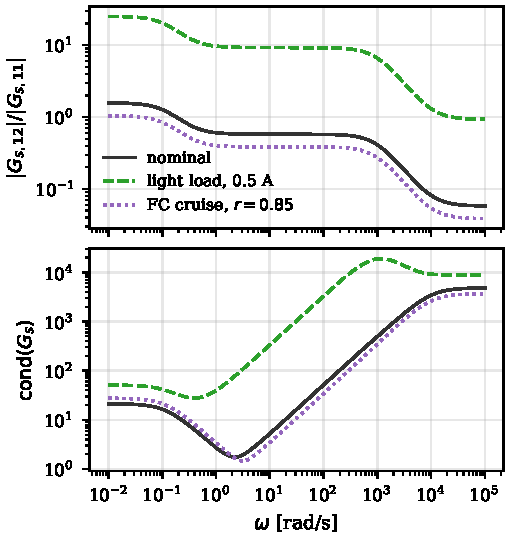
\includegraphics[width=\linewidth]{Figures/fig_coupling_sigma.pdf}
    \caption{Coupling versus frequency for three scenarios (nominal \SI{2}{\ampere} $r=0.5$;
    light load \SI{0.5}{\ampere}; FC cruise $r=0.85$). Top: directional ratio
    $|G_{s,12}(j\omega)|/|G_{s,11}(j\omega)|$ on the scaled plant. Bottom:
    $\mathrm{cond}(G_s(j\omega))$ for the same scenarios. All three curves reach or exceed unity
    in band and the light-load curve exceeds it by more than an order of magnitude: that is the
    whole motivation for considering a centralized design; the RGA is
    identically $I$ for all three and would show nothing.}
    \label{fig:coupling-sigma}
\end{figure}

\subsection{Operating envelope and validation}
\label{sec:envelope}

An operating point is the 4-tuple $\mathrm{OP} = (I_{tot0}, r_0, \Delta V_0, v_0)$, nominally
$I_{tot0} = \SI{2}{\ampere}$, $r_0 = 0.50$, $\Delta V_0 = +\SI{0.2}{\volt}$ and
$v_0 = \SI{2}{\meter\per\second}$; half the $\pm\SI{0.4}{\volt}$ budget is used for $\Delta V_0$
deliberately, since synthesizing at zero would show the controller no coupling at all and at
$\pm0.4$ would over-commit to one sign. The uncertainty families are 10 operating points, 24
share corners and 24 drive corners; of the $10\times24\times24 = 5760$ Tier-1 combinations,
\textbf{768 are infeasible} --- the unidirectional ideal-diode switches make \eqref{eq:share}
meaningless where it puts $\alpha_0$ outside $(0,1)$ --- and are skipped and counted instead of
silently linearized, leaving the \textbf{4992 feasible corners} used throughout. Synthesis and
all frequency-domain metrics run on the scaled plant $G_s = D_e^{-1} G D_u$ with
$D_e = \mathrm{diag}(0.05, 0.5)$ and $D_u = \mathrm{diag}(0.35, 20.0)$, giving
$G_s(0) = \left[\begin{smallmatrix} 7.0 & -11.03 \\ 0 & 148.3 \end{smallmatrix}\right]$ and
$\mathrm{cond}(G_s(0)) = 21.31$. Writing $K$ as \eqref{eq:K} rather than sweeping it makes the
SISO envelope $K\in[0.55,1.45]$ \emph{derived}, and exposes a gap: over the full feasible
operating set the implied envelope is $[0.533, 2.067]$, $43\,\%$ above it at light load with full
mismatch. Those corners are carried as stability-only corners. Full corner-family definitions,
feasibility arithmetic and envelope tables are in Appendix~\ref{app:corners}. The design plant is
independently checked against a 15-state converter-level truth model in which the coupling
\emph{emerges from the circuit} rather than being written in, agreeing to $0.032\,\%$ at DC and
within $0.93\,\%$ in band at nominal (Appendix~\ref{app:fullorder}).

%%%%%%%%%%%%%%%%%%%%%%%%%%%%%%%%%%%%%%%%%%
\section{The Two SISO Designs}
\label{sec:siso}

\subsection{Share controller}

The share half of the decentralized baseline is the existing firmware share controller
\citep{internal:droop}: an $H_\infty$/Youla-H design on the SISO share plant \eqref{eq:G11} with
$\gamma_{opt} = 0.6532$, built at a $5\,\%$ back-off ($\|T_{zw}\|_\infty = 0.6841$) and realized
as three biquads plus a trapezoidal integrator at \SI{1}{\kilo\hertz} with back-calculation
anti-windup. It achieves $T(0)=1$ exactly by the scalar Youla-H correction, an S/T crossover near
\SI{110}{\radian\per\second}, a nominal $M_2$ margin of \num{0.80}
(\citep{assadian2020neoclassical}, Def.~4.2 and Props.~4.2--4.3, pp.~148--149) with
\SI{73.9}{\degree} phase
margin, and a \SI{11.7}{\milli\second} delay margin --- roughly six times the worst modeled
delay. Against a 60-corner family it is stable everywhere with worst-corner discrete
$\|S\|_\infty = 1.87$, against \num{26.9} for the nominally tuned PI it replaced. It is used here
\emph{unchanged}.

\subsection{New SISO drive controller}

The drive half of the baseline did not exist and was built for this study, following the recipe
of \citep{tan2025scaling,tan2025youlah} on the drive plant \eqref{eq:G22}: a second-order
strictly-proper weight on $S$, a \texttt{makeweight} roll-off weight on $T$, and a control-effort
weight on $Y$. Two deviations were forced. The papers' $W_{\Delta}$ break at
\SI{18}{\radian\per\second} sits \emph{below} the $W_p$ corner on this plant, making the two
weights contend over the same decade, inflating $\gamma$ and collapsing the achieved crossover;
the break was moved to $2.5\times$ the $W_p$ corner, preserving the intent. Second, the achieved
crossover lands consistently \emph{below} the $W_p$
corner with $\gamma_{opt}\gg1$ throughout: \textbf{the specifications are being shaped, not met}.
The cause is that a second-order strictly-proper $S$ weight demands two integrators in the loop
below its corner, and the drive plant's mechanical pole at \SI{0.122}{\radian\per\second}
contributes none of them, leaving only the controller's single integrator; no reweighting brings
$\gamma$ below about $1.2$ (Appendix~\ref{app:driveweights}). $W_p$ was therefore cornered at
\SI{50}{\radian\per\second} to land the achieved crossover near the papers'
\SI{24}{\radian\per\second}, at $\gamma_{opt} = \num{13.03}$.

A $\gamma$ of \num{13.03} means the weights are not met; the controller itself is sound. The
delivered loop has $\|S\|_\infty = 1.3851$ nominal, \SI{48.9}{\degree} phase margin at
\SI{20.75}{\radian\per\second}, \SI{18.3}{\decibel} gain margin and a \SI{41.12}{\milli\second}
delay margin, and is stable at all 72 drive corners with worst continuous
$\|S\|_\infty = 2.4074$. The scalar Youla-H correction is tiny here ($T_H(0) = 0.99864$, a gain
scale of \num{1.00137}) and delivers $T(0) = 1.000000000000$.

Anti-windup drives the cost comparison of
Section~\ref{sec:implementation}. The reduced controller's \emph{non-integral} branch alone has a
DC gain of \SI{367.7}{\ampere\per\meter\per\second}, so it saturates the $\pm\SI{20}{\ampere}$
actuator for speed errors above $e_{sat} = \SI{54.4}{\milli\meter\per\second}$ and its lag states
wind up independently of the integrator. The failure is therefore \emph{amplitude-bounded}. A step-amplitude scan of
the integrator-only back-calculation scheme (pass: final error below
$\SI{e-4}{\meter\per\second}$ and tail peak-to-peak below $\SI{e-5}{\meter\per\second}$) is clean
at $0.02$, $0.05$, $0.10$ and \SI{0.20}{\meter\per\second} --- final errors of order
$\SI{e-8}{\meter\per\second}$ --- and fails from \SI{0.5}{\meter\per\second} upward, reaching a
\SI{-0.101}{\meter\per\second} standing error and a \SI{6.3}{\milli\meter\per\second} limit cycle
on the 0 to \SI{2}{\meter\per\second} step. \textbf{Integrator-only conditioning is adequate for
small transients and inadequate for large ones}; since the 0 to \SI{2}{\meter\per\second} step is
a required gate, the baseline still \emph{requires} Hanus
self-conditioning \citep{hanus1987conditioning} on a five-state state-space realization
(Appendix~\ref{app:aw}), which is \emph{not} implementable as a biquad cascade.

%%%%%%%%%%%%%%%%%%%%%%%%%%%%%%%%%%%%%%%%%%
\section{Centralized $2\times2$ $H_\infty$ / Youla-H Synthesis}
\label{sec:mimo}

\subsection{Weights and the DGKF solution}

Synthesis uses block-diagonal weights on the three-block stack
$[\,W_p S;\; W_u Y;\; W_{\Delta} T\,]$, one philosophy per channel
(Table~\ref{tab:mimo-weights}). This is the \emph{loop shaping} problem in the sense of
\citep{assadian2020neoclassical} \S6.4, eqs.~(6.44)--(6.48), pp.~229--232 (SISO) and \S14.5,
eq.~(14.67) and Fig.~14.20, p.~468 (MIMO), whose Youla-based formulation is the method this
report follows; \citep{zhou1996robust,skogestad2005multivariable} are complementary
references for the same machinery.\footnote{The wider literature often calls this three-block
form ``mixed-sensitivity $S/KS/T$''. We follow \citep{assadian2020neoclassical}, which reserves
\emph{mixed sensitivity} for the two-block $S/T$ problem (\S6.6, \S14.5) and calls the
three-block form loop shaping.} The share block is the SISO set of Section~\ref{sec:siso},
unchanged. The drive block is \emph{not} the Section~\ref{sec:siso} set --- it was iterated
independently against the MIMO corner battery (Appendix~\ref{app:driveweights}) --- and that
difference bounds how the two designs may be compared (Section~\ref{sec:fairness}). The binding
constraint on this plant turns out to be corner robustness instead of nominal performance, so
\textbf{$\gamma$ is the wrong scalar to minimize here}: the final drive block deliberately accepts
a worse $\gamma$ than an available alternative in exchange for corner margin, paying about
\SI{60}{\milli\second} of small-signal drive settling.

\begin{table}[H]
\caption{Final block-diagonal weights. Bandwidth separation (share $\approx$
\SI{110}{\radian\per\second} vs.\ drive \SI{24}{\radian\per\second}) is deliberate: the share
loop rides on \SI{1}{\milli\second} electrical dynamics, the drive loop on an \SI{8}{\second}
mechanical mode. All $\gamma$ values are a-posteriori achieved levels.}
\label{tab:mimo-weights}
\begin{tabularx}{\textwidth}{lXX}
\toprule
\textbf{Block} & \textbf{Share channel} & \textbf{Drive channel} \\
\midrule
$W_p$ (on $S$) & \texttt{strictly\_proper\_lf}$(10^4, 40)$ & \texttt{strictly\_proper\_lf}$(10^4, 24)$ \\
$W_{\Delta}$ (on $T$) & \texttt{makeweight}$(0.5, 250, 40)$ & \texttt{makeweight}$(0.5, 60, 40)$ \\
$W_u$ (on $Y$) & \texttt{makeweight}$(0.3, 600, 20)$ & \texttt{makeweight}$(0.5, 18, 20)$ \\
\midrule
\multicolumn{2}{l}{$\gamma$: share alone / drive alone / MIMO} & 0.5760 / 1.6429 / \textbf{1.6456} \\
\bottomrule
\end{tabularx}
\end{table}

The augmented plant has 14 states with $p_z = 6$, $p_y = 2$, $m_u = 2$, and is solved by the
two-Riccati DGKF construction \citep{doyle1989state} (equivalently
\citep{assadian2020neoclassical} \S15.3, Thm.~15.2, eqs.~(15.94)--(15.98), pp.~491--493). The
same source's Remark on p.~492 --- that a control input carrying no weight breaks the $D_{12}$
rank condition --- is why $W_u$ is non-empty on both channels: it is a solvability requirement,
not a tuning preference. Two features of the solution bear on
every $\gamma$ in this report. First, the measurement-equals-reference structure
gives $D_{21} = I_2$, which makes the filter Riccati degenerate with $P_f \equiv 0$ as the
provably stabilizing solution --- reproduced to $\SI{1.0e-14}{}$, which serves as a correctness
check on the estimation half of the solver at no additional cost. Second, because $P_f\equiv0$ the DGKF feasibility test
$\rho(P_c P_f)<\gamma^2$ is vacuous, so the Riccati bisection is optimistic in MIMO and must not be
gated on: it reports $\gamma = 0.89769$ while the central controller attains
$\gamma_{achieved} = \mathbf{1.64563}$ with $\|T_{zw}\|_\infty = 1.64573$. \textbf{Every $\gamma$
quoted in this report is an a-posteriori achieved level.} Details and formulas are in
Appendix~\ref{app:dgkf}.

Because $G_{21}=0$, any MIMO controller restricted to
$e_1 = 0$ acts as a drive-channel SISO controller, so $\gamma_{MIMO} \ge \gamma_{drive}$
necessarily; measured, $1.6456 \ge 1.6429$, equal to $0.16\,\%$: \textbf{the coupling costs
essentially nothing}, since the centralized controller
attains the drive channel's own unconstrained optimum while also handling $G_{12}$. And at
$\Delta V_0 = 0$ the plant is exactly diagonal, so the problem must decouple and
$\gamma_{MIMO} = \max(\gamma_{share}, \gamma_{drive})$; measured, \num{1.64187} vs.\
\num{1.64295} --- $0.07\,\%$ on a case with a known closed-form answer.

\subsection{The MIMO Youla-H DC correction: $T(0)=I$}
\label{sec:youlah}

This is the report's control-theoretic contribution. $T(0)=I$ is the MIMO statement of perfect
low-frequency tracking, zero steady-state error and input--output decoupling
(\citep{assadian2020neoclassical} \S12.7.1, p.~414), recognizable by
$\bar\sigma(T) = \sigma_{\min}(T) = 1$ at low frequency; its SISO ancestor is the interpolation
condition $G_p(0)Y(0) = T(0) = 1$ of \S3.4, eq.~(3.64), p.~113, which the matrix correction below
generalizes. The Youla route of
\citep{assadian2020neoclassical} enforces $T(0)=1$ \emph{by construction}, as an interpolation
condition imposed while $Y$ is shaped (\S3.5); $H_\infty$ synthesis honours no interpolation
conditions natively, so it delivers a controller that is only approximately integral. The
correction here therefore restores post-synthesis a property that the book's own route obtains
by construction --- it is a repair, not a new capability. For a SISO plant $G_P$, the recipe of
\citep{tan2025youlah} takes the $H_\infty$-synthesized Youla parameter in zero-pole-gain form,
\begin{equation}\label{eq:YH}
Y_H(s) = K_H \frac{\prod_{i=1}^{n}(s+z_i)}{\prod_{j=1}^{m}(s+p_j)},
\end{equation}
keeps every $z_i$ and $p_j$, and rescales the gain alone to $K_{YH} = K_H/(Y_H(0)G_P(0))$, which
enforces $T_{YH}(0) = G_P(0)Y_{YH}(0) = 1$ and, since $G_C = Y/S$ and $S(0)=0$, plants at least
one pure integrator in the realized controller.

A scalar gain has no matrix analogue that preserves ``the same zeros and poles.'' But it has one
that preserves the \emph{dynamics}: a constant \emph{right} multiplier. Build the Youla parameter
by state-space interconnection, $Y_H = K_H(I + G_s K_H)^{-1}$, valid because $D_K = 0$, so that
$T = G_s Y_H$ exactly as in the scalar case. Then define
\begin{equation}\label{eq:M}
M_{YH} \;:=\; \left[G_s(0)\,Y_H(0)\right]^{-1} \in \mathbb{R}^{2\times2},
\qquad
Y_{YH}(s) \;:=\; Y_H(s)\,M_{YH} .
\end{equation}
Since $M_{YH}$ multiplies only the input matrix of the state-space realization, the poles and zero
dynamics of $Y_H$ are untouched --- the exact matrix analogue of ``keep $z_i$ and $p_j$, change
$K$.'' The correction is immediate:
\begin{equation}\label{eq:T0}
T_{YH}(0) \;=\; G_s(0)\,Y_{YH}(0) \;=\; G_s(0)\,Y_H(0)\left[G_s(0)Y_H(0)\right]^{-1} \;=\; I .
\end{equation}
The scalar recipe is recovered exactly when the problem is $1\times1$:
$M_{YH} = 1/(G_P(0)Y_H(0))$,
i.e.\ $K_{YH} = K_H/(Y_H(0)G_P(0))$.

The choice of \emph{right} multiplication is forced twice over. Algebraically, $T = G_s Y$, so
only a right factor of $Y$ can be inverted against $G_s(0)Y_H(0)$ to give the identity;
$M_{YH}\,Y_H$
would give $G_s(0)M_{YH}\,Y_H(0)\ne I$ in general because matrices do not commute. Physically,
left-multiplying would mix the controller \emph{outputs} rather than re-map its inputs, changing
which actuator answers which error --- yielding a different controller instead of a corrected one.

The realization follows the scalar case block-for-block:
$G_{c,YH} = Y_{YH}(I - G_s Y_{YH})^{-1}$, a positive feedback of $G_s$ around $Y_{YH}$,
well-posed because $D_Y = 0$. The final step is what makes the property robust rather than merely
achieved: an ordered real Schur decomposition plus Sylvester block-diagonalization separates the
two near-origin poles of $G_{c,YH}$ into an exact residue bank $K_I/s$ plus a stable remainder.
\textbf{After the split, $T(0)=I$ is structural} --- two exact integrators with a non-singular
$K_I$ force $S(0)=0$ regardless of any subsequent rounding, truncation or float32 quantization,
so the DC property no longer depends on a numerically delicate pole-at-almost-zero, which is the
risk the scalar recipe carries into a fixed-point implementation. Numerically,
\begin{equation}\label{eq:KI}
K_I = \begin{bmatrix} \phantom{-}7.992467 & 0.1645500 \\ 7.8\times10^{-5} & 0.1031860 \end{bmatrix},
\end{equation}
nearly lower triangular with a small $(1,2)$ entry and a negligible $(2,1)$ entry: the DC
coupling correction runs drive$\,\to\,$share, matching the plant's triangularity.

The correction is a small adjustment rather than a substantial repair. Here
$\mathrm{cond}(G_s(0)Y_H(0)) = 1.0001$ --- the book's low-frequency decoupling recognizer
$K(T_y)\approx1$ (\citep{assadian2020neoclassical} \S12.8.1, p.~416) --- and
$\|M_{YH} - I\|_2 = \SI{1.57e-4}{}$, saying the $H_\infty$
controller was already integral to four decimals, as one expects from an $S$ weight with DC gain
$10^4$ (a large $\|M-I\|$ would have implicated the weights themselves).
The delivered $\|T(0)-I\|_{\max}$ is $\SI{6.5e-10}{}$, preserved through reduction. The
correction's remaining job is therefore not to \emph{create} the integrator --- $H_\infty$ already
put a near-integrator there --- but to fix its \emph{direction}.

\subsubsection{Relation to the direct MIMO Youla design route}
The plant here is stable and square, so its Smith--McMillan structure imposes no unstable
pole/zero interpolation constraints and the direct MIMO Youla design of
\citep{assadian2020neoclassical} \S13.2 (pp.~422--425) applies verbatim, with the controller
recovered as $Y = G_p^{-1}T_{yd}$ and $G_c = Y S_y^{-1}$ (\S13.5, p.~445). It was not used here
because the binding constraint on this problem is robustness across the corner family rather
than nominal shaping: $H_\infty$ synthesis optimizes a worst-case norm directly, whereas the
direct route would require the designer to guess a $T_{yd}$ that survives all 4992 corners.
The Youla-H correction above then re-imposes the one property the direct route would have given
by construction.

\subsection{Utilization of the cross-coupling by the centralized controller}

Table~\ref{tab:K-entries} quantifies the extent to which the centralized controller uses the
cross-coupling.

\begin{table}[H]
\caption{Peak scaled magnitude of each controller entry, and its ratio to the diagonal term of
the same row.}
\label{tab:K-entries}
\begin{tabularx}{\textwidth}{lCC}
\toprule
\textbf{Entry} & \textbf{Peak $|\cdot|$ (scaled)} & \textbf{Ratio to its diagonal} \\
\midrule
$K_{11}$ (share $\leftarrow$ share error) & 79.92 & --- \\
$K_{12}$ (share $\leftarrow$ speed error) & \textbf{1.7167} & \textbf{2.15\,\%} \\
$K_{21}$ (drive $\leftarrow$ share error) & $9.93\times10^{-4}$ & 0.074\,\% \\
$K_{22}$ (drive $\leftarrow$ speed error) & 1.3345 & --- \\
\bottomrule
\end{tabularx}
\end{table}

$K_{21}\approx0$ is correct and expected: $G_{21}=0$, so there is nothing the drive actuator can
do about a share error, and its $\SI{7.4e-4}{}$ ratio is numerical residue --- a check
that the synthesis recovers the plant's triangularity. $K_{12}$ at $2.15\,\%$ of
$K_{11}$ is the real coupling feedforward: the share actuator pre-empts the bus-current
disturbance a commanded acceleration is about to create. It is small in \emph{ratio} because
$K_{11}$ must be large (the share loop's \SI{110}{\radian\per\second} bandwidth); the
term itself is fully active. Its magnitude is bounded by the $\Delta V_0$ sign uncertainty by construction:
a feedforward built at $+\SI{0.2}{\volt}$ is the wrong sign at $-\SI{0.4}{\volt}$, and the
synthesis assigns it little authority.

\textbf{The centralized controller is about $98\,\%$ decentralized by gain.} Decentralized
control here is therefore justified on its merits, on the centralized design's
own evidence.

%%%%%%%%%%%%%%%%%%%%%%%%%%%%%%%%%%%%%%%%%%
\section{Implementation}
\label{sec:implementation}

The order-30 controller $G_{c,YH}$ reduces, after the exact integrator split and balanced
truncation at a $10^{-2}$ margin, to \textbf{9 continuous states}: two exact integrators plus a
seven-state remainder, with a maximum relative $\bar\sigma$ deviation of $\SI{1.88e-3}{}$ over
$\omega\in[0.1,10^4]$ against a $2\times10^{-2}$ tolerance. The order is set by the Hankel
spectrum: the singular-value tail is flat here (states 6 and 7 carry
$\SI{9.2e-4}{}$ and $\SI{6.3e-4}{}$ against a leading \num{0.45}), so truncating at five would
not clear the $10^{-2}$ auto-selection margin. \textbf{The selection tolerance was deliberately
not loosened to force a smaller controller}: two float32 states cost 8 bytes and about 26 MAC
per tick, whereas a corner result that survives only because truncation error happened to damp
the worst corner is not a design property at all (Appendix~\ref{app:driveweights}). The whole
controller runs single-rate
at \textbf{\SI{2}{\milli\second} (\SI{500}{\hertz})}, because it issues the motor current command
and the VESC UART frame floor caps that channel there; the cost to the share channel is bounded
and checked explicitly, since Nyquist at \SI{1571}{\radian\per\second} is still
$14\times$ the \SI{110}{\radian\per\second} share crossover --- which is what discharges the
standing assumption that discretization has no performance effect at a reasonable sampling rate
(\citep{assadian2020neoclassical}, p.~261) --- and the extra effective delay of at
most \SI{1}{\milli\second} sits inside the SISO design's \SI{11.7}{\milli\second} delay margin.
The entire Tier-1 family is re-verified in discrete time (0 of 4992 unstable). Discretization
(exact $2\times2$ Tustin integrator, real-modal remainder) and the matrix-valued anti-windup
scheme are detailed in Appendix~\ref{app:aw}.

\begin{table}[H]
\caption{Implementation on the Teensy 4.1 (600\,MHz Cortex-M7). The decentralized state count is
quoted as implemented: its drive half needs a six-state Hanus self-conditioned realization rather
than the five-state controller order, because the conditioning product adds a state's worth of
storage and an $n^2$ term per tick. The MIMO MAC figure counts the state-space core
($Ax + Be$, $Cx + De$, integrator) only, which is the same basis on which the decentralized
halves are counted; counting the $D_e^{-1}/D_u$ scaling and the back-calculation arithmetic as
well gives \num{97} MAC per tick (\SI{48500}{} MAC per second) for the same code. Both
accountings are quoted in the design record; only the like-for-like one belongs in a ratio.}
\label{tab:cost}
\begin{tabularx}{\textwidth}{lCC}
\toprule
\textbf{Quantity} & \textbf{Decentralized} & \textbf{MIMO} \\
\midrule
rate & \SI{1}{\kilo\hertz} (share) $+$ \SI{500}{\hertz} (drive) & \SI{500}{\hertz} single-rate \\
controller states (implemented) & $4 + 6 = \mathbf{10}$ & \textbf{9} \\
anti-windup & scalar back-calculation $+$ Hanus & $D_u^{-1}$ back-calculation $+$ clamp \\
MAC per tick & $18$ @ \SI{1}{\kilo\hertz}, $63$ @ \SI{500}{\hertz} & $89$ @ \SI{500}{\hertz} \\
\textbf{MAC per second} & \textbf{49\,500} & \textbf{44\,500} \\
ratio MIMO / dec & --- & \textbf{0.899} \\
coefficient floats & --- & 101 (404\,B) \\
float32 replay error (64-step, saturating) & --- & $\SI{5.52e-6}{}$ (tol.\ $\SI{5e-4}{}$) \\
\bottomrule
\end{tabularx}
\end{table}

\textbf{The two are comparably inexpensive, with the
centralized controller slightly ahead}, at $0.899\times$ the decentralized MAC rate and one fewer
state. It is ahead at all only because the decentralized baseline \emph{cannot} be a biquad
cascade --- its drive half needs the Hanus state-space form, whose $A_d - B_d C_d/D_d$ product
costs an extra $n^2$ per tick, and it runs one of its two halves at \SI{1}{\kilo\hertz}. A
$10\,\%$ margin is not an argument for either architecture:
\textbf{compute cost does not discriminate here}. Both figures are
negligible on this core (under $0.1\,\%$ of a single issue slot), so \textbf{the compute cost is
not the cost}. The genuine costs of centralization are that it moves the share loop from
\SI{1}{\kilo\hertz} to \SI{500}{\hertz} and couples the two control tasks into one scheduling
unit; float32 coefficient sensitivity; and a matrix-valued anti-windup scheme that is more code
to get right than the scalar one. The UART frame floor is unchanged either way and remains the
true bottleneck.

\subsection{Actuator rate limiting of the drive channel}
With $K_F = k_t\eta_{dt}\varphi/r_t = \SI{1.334}{\newton\per\ampere}$ and
$m_{\!e\!f\!f} = \SI{2.95}{\kilo\gram}$, the $\pm\SI{20}{\ampere}$ clamp bounds acceleration at
$a_{max} = \SI{9.04}{\meter\per\second\squared}$: no reference the loop can be asked to follow is
tracked faster than that, whatever the design bandwidth says. The share step (0.05 share) settles
to $2\,\%$ in \SI{44}{\milli\second} and the small-signal drive step
(\SI{0.05}{\meter\per\second}, peak \SI{1.18}{\ampere}) in \SI{150}{\milli\second}, both with
exact final values. A \SI{0.5}{\meter\per\second} step is also linear at this clamp --- its
\SI{11.79}{\ampere} peak sits inside the rail --- and settles in \SI{150}{\milli\second} to
\num{0.500000}. The clamp binds from roughly \SI{1}{\meter\per\second} of step amplitude upward,
which is where the large-signal cases of Section~\ref{sec:comparison} live. \textbf{The
\SI{24}{\radian\per\second} bandwidth is still a small-signal claim}; it now holds over a usefully
wider amplitude range than the anti-windup boundary
$e_{sat} = \SI{54.4}{\milli\meter\per\second}$ of the decentralized drive half.

%%%%%%%%%%%%%%%%%%%%%%%%%%%%%%%%%%%%%%%%%%
\section{Comparison}
\label{sec:comparison}

\subsection{Setup and fairness conditions}
\label{sec:fairness}

Three controllers are compared. \texttt{dec} is the decentralized baseline,
$\mathrm{blkdiag}(K_{share}, K_{drive})$, with the share controller at \SI{1}{\kilo\hertz} and
the Section~\ref{sec:siso} drive controller at \SI{500}{\hertz}. \texttt{mimo} is the
Section~\ref{sec:mimo} controller at \SI{500}{\hertz}. \texttt{dec500} is the decentralized pair
with its share half re-discretized at \SI{500}{\hertz}, and exists purely to isolate the
sample-rate difference as a confound --- it changes the share excursion by $0.8\,\%$ (large step)
and $7.1\,\%$ (small step), leaves the regen bus excursion bit-identical and Tier-1 stability at
0/4992, so \textbf{every conclusion below survives equalizing the sample rates}.

The essential fairness condition is that \textbf{both controllers are closed against the same
coupled $2\times2$ plant}, using the same assembly routine, corner sets and simulations; the
decentralized controller is never evaluated on a diagonal plant, which would bias the
comparison in its favour by construction. Time-domain results use a multirate discrete simulator at a
\SI{0.1}{\milli\second} base step with the plant ZOH-discretized per corner, so \texttt{dec} runs
its two halves at their native rates; frequency-domain results use continuous
physical-coordinate controllers recovered from the emitted float32 headers by exact inverse
Tustin plus the analytic $K_I/s$ integrator. All time-domain signals are small-signal deviations
about the nominal operating point.

\subsubsection{Corner-family verification in place of a small-gain certificate}
The robustness certificate of \citep{assadian2020neoclassical} is the small-gain condition
$\bar\sigma(W_{\Delta}T_o) < 1$ against a norm-bounded multiplicative perturbation (\S14.5,
Thm.~14.3, p.~466). This study does not use it. The dominant uncertainties here --- the
\emph{sign} of $\Delta V_0$, the structural gain multiplier $K_v$, and the transport delays ---
are parametric and structured, and wrapping them in an unstructured norm bound large enough to
cover the $\Delta V_0$ sign flip would be so conservative that no controller would certify.
Robustness is therefore verified by explicit evaluation over the parametric corner family.
\textbf{$W_{\Delta}$ in this report is a shaping filter,
not an identified uncertainty bound}, and \textbf{no claim of $\bar\sigma(W_{\Delta}T_o) < 1$ is
made or implied} by any $\gamma$ quoted here.

A further limitation: the two designs use different weight
\emph{families} on the drive channel (second-order at \SI{50}{\radian\per\second} for the SISO
baseline, first-order at \SI{24}{\radian\per\second} for the MIMO) and their $\gamma$ values sit
on different plant scalings, so \textbf{$\gamma$ is not comparable between them and is never
quoted side by side}. Which controller performs better on the real coupled plant is settled by
the closed-loop harness regardless.

\subsection{The three primary metrics give three different answers}

\begin{table}[H]
\caption{The three primary metrics and their verdicts. Worst-corner sensitivity is the Tier-2
in-envelope $\bar\sigma(S_o)$; excursions are small-signal
($\Delta v_{ref} = +\SI{0.05}{\meter\per\second}$, zero time on the current rail).}
\label{tab:headline}
\begin{tabularx}{\textwidth}{XCCX}
\toprule
\textbf{Metric} & \texttt{dec} & \texttt{mimo} & \textbf{Verdict} \\
\midrule
worst-corner $\|S\|_\infty$ (in-envelope $\bar\sigma(S_o)$) & 2.5535 & \textbf{1.8754} & \textbf{MIMO superior}, $-27\,\%$ (both on the same representative corner set) \\
drive-transient share excursion, $\Delta V_0 = +0.4 / -0.4$ & 0.01744 / 0.01744 & \textbf{0.00667} / 0.01935 & \textbf{split by $\Delta V_0$ sign} ($-62\,\%$ / $+11\,\%$) \\
regen-event bus excursion & \SI{1.49112}{\volt} & \SI{1.47429}{\volt} & \textbf{tie} (ratio 0.989) \\
\bottomrule
\end{tabularx}
\end{table}

\subsubsection{Metric 1: worst-corner sensitivity}
At the nominal plant the centralized controller has $\|S_o\|_\infty = 1.2287$ against $1.3974$,
and over the Tier-2 in-envelope family its worst $\bar\sigma(S_o)$ is \num{1.8754} against
\num{2.5535}, better at \textbf{167 of 168 corners} (Figure~\ref{fig:sigma-S-both};
full tables and the per-corner scatter in Appendix~\ref{app:corners}). Two qualifications attach
to the absolute numbers. The Tier-2 figure is computed on a representative corner subsample, so
it is a lower bound on the full-grid worst and an absolute ``$<2.0$'' target read off it is
subsample-dependent --- but the decentralized comparison point comes from the same set, so the
\emph{relative} $27\,\%$ verdict stands. And the $195\times$ nominal improvement in the
cross-transfer $\|T_{\alpha\leftarrow v_{ref}}\|_\infty$ (\num{0.25676} against
$\SI{1.314e-3}{}$) is a continuous-domain figure: on the as-implemented
\SI{2}{\milli\second} loop it is $\SI{1.109e-2}{}$, about $\mathbf{23\times}$ better than
decentralized. Both controllers are stable at 0 of 4992 Tier-1 corners unstable, in continuous
time and in the exact multirate discrete loop --- \textbf{no decentralized instability was found
anywhere}.

\begin{figure}[H]
    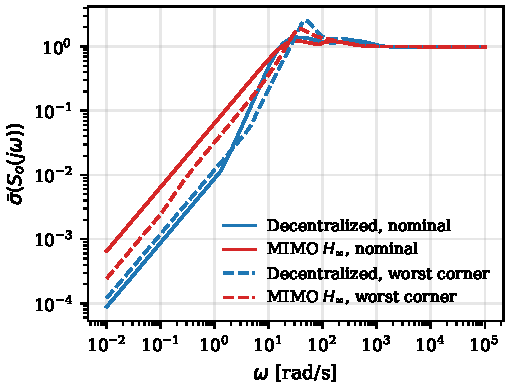
\includegraphics[width=\linewidth]{Figures/fig_sigma_S_both.pdf}
    \caption{$\bar\sigma(S_o(j\omega))$ for both controllers, at the nominal operating point and
    at the worst in-envelope corner ($I_{tot0} = \SI{2}{\ampere}$, $r_0 = 0.3$,
    $\Delta V_0 = \SI{-0.4}{\volt}$, with the drive channel's gain and delay extremes). Blue is
    decentralized, red is MIMO $H_\infty$.}
    \label{fig:sigma-S-both}
\end{figure}

\subsubsection{Metric 2: drive-transient share excursion}
At the sign of $\Delta V_0$ the centralized
controller was synthesized for, it cuts the drive-induced share excursion by $62\,\%$ and settles
faster (\SI{0.175}{\second} against \SI{0.189}{\second}) with a $43\,\%$ smaller current peak; at
the mirrored sign it makes the excursion $11\,\%$ worse (Figure~\ref{fig:transient-small}) --- a
downside that is now marginal rather than punitive. The
decentralized traces are identical between the two signs --- as they must be, since a diagonal
controller on a linear plant sees only the magnitude of the coupling and is blind to its sign. Splitting the
corner statistics by sign over the 96 coupled in-envelope corners, the median cross-transfer
ratio MIMO/dec is \textbf{0.941} when the sign matches the synthesis and \textbf{2.162} when it
opposes, spread $0.1938$ to $4.378$; the centralized controller has the smaller cross-transfer at
28 of 96 corners. \textbf{The $\approx2.3\times$ asymmetry between the matching and opposing
medians is insensitive to the actuator span and the operating point}, where the magnitude of the
benefit is not. The saturated large step
($+\SI{2}{\meter\per\second}$) splits by sign in the same way --- the centralized controller is
$48\,\%$ better at the matching sign and $90\,\%$ worse at the opposing one --- and the
decentralized pair reaches a droop clamp ($r = 0.85$ at $\Delta V_0 = +0.4$, $r = 0.15$ at
$-0.4$) at both signs, whereas the centralized one reaches a clamp only at the matching sign
(Appendix~\ref{app:corners}). What the decentralized pair keeps outright there is \emph{speed}
recovery: it settles $45\times$ faster after the saturation episode, because the centralized
drive integrator residue is only $K_{I,22} = 0.103$ against a \SI{0.122}{\radian\per\second}
vehicle pole, so post-saturation recovery is slow \emph{by design}.

\begin{figure}[H]
    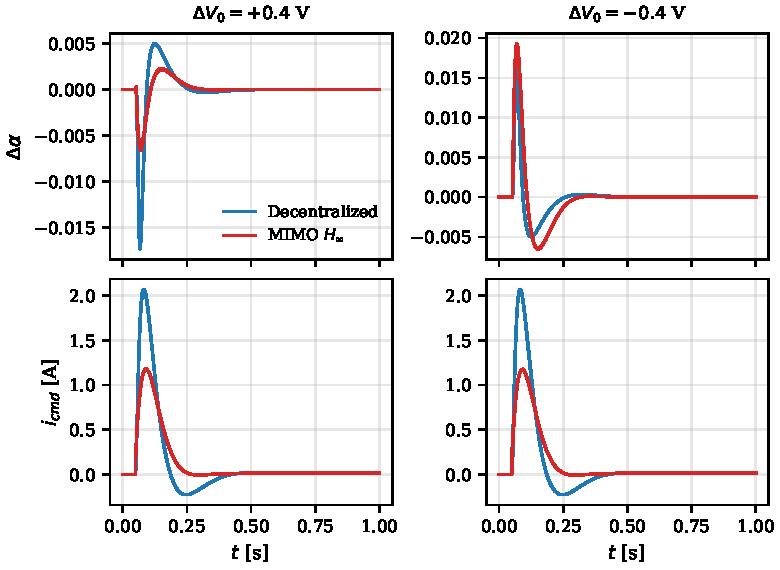
\includegraphics[width=\linewidth]{Figures/fig_transient_small.pdf}
    \caption{Small-signal drive transient, $\Delta v_{ref} = +\SI{0.05}{\meter\per\second}$
    (zero time on the current rail). Left column $\Delta V_0 = +\SI{0.4}{\volt}$, right column
    $\Delta V_0 = -\SI{0.4}{\volt}$; top row share deviation, bottom row motor current command.
    The first \SI{1}{\second} of the \SI{12}{\second} simulation is shown; both responses are in
    steady state for the remainder. The decentralized traces are identical between columns while
    the centralized traces invert.}
    \label{fig:transient-small}
\end{figure}

\subsubsection{Metric 3: regen bus excursion}
Run against the 15-state truth model with $i_{cmd}$ railing at $-\SI{20}{\ampere}$, the bus
excursion is \SI{1.4911}{\volt} against \SI{1.4743}{\volt}, a ratio of \num{0.989}:
\textbf{essentially controller-independent}. The event is \emph{not} rail-dominated --- the current command
spends only $0.18$ to $0.34\,\%$ of the horizon on the clamp --- so ``both controllers sit on the
same rail'' does not account for the tie. What accounts for it is that the bus excursion is set
by the \emph{peak braking current the loop reaches}, and both controllers reach essentially the
same peak on the same $-\SI{2}{\meter\per\second}$ demand; the droop loop, whatever its
architecture, has no authority over a disturbance injected downstream of it on that timescale.
This metric was proposed as an architecture discriminator \citep{internal:droop};
\textbf{it is not one} --- it measures the excitation, not the controller. On the same event the
centralized controller is the better of the two on share excursion ($0.1448$ against $0.1747$)
and recovers the bus faster (\SI{0.43}{\second} against \SI{0.58}{\second})
(Appendix~\ref{app:corners}).

\subsubsection{Input sensitivity $\bar\sigma(S_u)$}
For a MIMO plant, output sensitivity does not bound input sensitivity: $S_u = (I+G_cG_p)^{-1}$
and $S_y = (I+G_pG_c)^{-1}$ differ whenever the plant condition number differs from unity, and
the available bound (\citep{assadian2020neoclassical} \S12.7.2, eqs.~(12.86)--(12.87), p.~416)
only gives $\bar\sigma(S_u) \le K(G_p)\,\bar\sigma(S_y)$. That is a live concern here, since
$\mathrm{cond}(G_s)$ is \num{21.31} at DC and peaks near \num{8835} in band
(Table~\ref{tab:coupling}), so the loose bound admits input sensitivities three orders of
magnitude above the output ones. Direct evaluation (same continuous controller assembly as every
other frequency metric in this report) shows the bound is far from tight:

\begin{table}[H]
\caption{Input sensitivity $\bar\sigma(S_u)$, peak value and the frequency at which it occurs.
Worst corner is $\Delta V_0 = \SI{-0.4}{\volt}$, $T_d = \SI{2}{\milli\second}$,
$\tau_r = \SI{300}{\micro\second}$, $\tau_f = \SI{0.8}{\milli\second}$, $K_v = 2$, damping
factor 2, $\tau_v = \SI{0.5}{\milli\second}$, $T_{d,v} = \SI{4}{\milli\second}$.}
\label{tab:su}
\begin{tabularx}{\textwidth}{XCC}
\toprule
\textbf{Case} & \texttt{dec} & \texttt{mimo} \\
\midrule
nominal, peak $\bar\sigma(S_u)$ & 1.3852 @ \SI{35.5}{\radian\per\second} & \textbf{1.2385} @ \SI{33.1}{\radian\per\second} \\
worst corner, peak $\bar\sigma(S_u)$ & 1.8640 @ \SI{54.6}{\radian\per\second} & \textbf{1.4749} @ \SI{41.3}{\radian\per\second} \\
\bottomrule
\end{tabularx}
\end{table}

Both controllers keep the realized input sensitivity modest --- comparable to their output
sensitivities rather than to the $K(G_p)$-scaled bound --- and the centralized controller is
again the better of the two, by $11\,\%$ nominally and $21\,\%$ at the worst corner. \textbf{The
input node raises no new concern for either architecture}; the decentralized baseline's
output-sensitivity deficit does not appear as an additional cost at the actuator.

\subsubsection{Caveats}
Six qualifications bound the above, expanded in Appendix~\ref{app:corners}. (i) The
$\Delta V_0$ sign uncertainty bounds any feedforward benefit: the entire centralized coupling
advantage lives in \eqref{eq:dalpha}, zero at $\Delta V_0 = 0$ and sign-flipping with it. (ii)
The $K$-out-of-envelope corners are waived; both controllers degrade badly there
($\bar\sigma(S_o) = 4.93$ centralized against $5.77$ decentralized). (iii)
The large steps and drive-cycle ramps still touch the clamp, so those comparisons are partly
about anti-windup recovery rather than linear design. (iv) The Tier-2 worst-corner numbers are a
representative subsample; the relative verdict survives, the absolute value does not. (v) In the
FC-charge-cruise regime the droop ratio is parked on its upper clamp and neither controller shows
windup interaction. (vi) \textbf{Nothing here is bench-calibrated}: $\Delta V_0$ above all,
plus $k_t$, the encoder chain, $m_{\!e\!f\!f}$, $\tau_v$ and $T_{d,v}$ remain open, and a
calibrated plant could move the verdicts, particularly the second metric.

%%%%%%%%%%%%%%%%%%%%%%%%%%%%%%%%%%%%%%%%%%
\section{Conclusions and Future Work}
\label{sec:conclusions}

\begin{enumerate}
\item \textbf{The coupling is real, one-directional, and operating-point dominated.} The droop
      ratio does not move the wheel speed ($G_{21}\equiv0$, a modelling result with its residual
      measured at $0.44\,\%$ of the bus), so the plant is exactly upper triangular and the RGA is
      identically $I$ at every frequency and corner. The live path is drive to share, through
      $\partial\alpha/\partial I_{tot} = -\Delta V_0 r_0(1-r_0)/(k_d I_{tot0}^2)$, at
      $1.57\times$ the direct path at \SI{2}{\ampere} and $25\times$ it at \SI{0.5}{\ampere} on
      the normalized plant. \textbf{The RGA is the wrong instrument for this plant.}
\item \textbf{Decentralized control is justified, not merely convenient.} It is stable at all
      4992 feasible Tier-1 corners, continuous and in the exact multirate discrete loop; it keeps
      a $2.3\times$ whole-cycle speed-tracking advantage and a $45\times$ faster recovery from
      saturation; it incurs a bounded penalty in worst-corner sensitivity ($2.55$ vs.\ $1.88$ on the
      same corner set); and none of its advantages depend on an uncalibrated sign. The
      centralized controller's own gains say the same thing from the other side --- it is about
      $98\,\%$ decentralized, with a $2.15\,\%$ coupling feedforward that the synthesis
      deliberately keeps small because it cannot trust the coupling's sign.
\item \textbf{The three primary metrics give three different answers}: the centralized
      controller is superior on worst-corner
      sensitivity by $27\,\%$, ties on regen bus excursion (a metric that measures the
      excitation rather than the controller and should be retired), and is superior or inferior
      on the drive-transient share excursion depending on
      the sign of $\Delta V_0$ --- with a median penalty ratio $\approx2.3\times$ between the
      opposing and matching signs. \textbf{The decentralized pair is not
      superior in every saturated large-signal case}: the large-signal share excursion splits by $\Delta V_0$ sign
      exactly as the small-signal one does. What decentralized retains outright is drive-cycle
      tracking, post-saturation recovery speed, and sign-independence.
\item \textbf{The MIMO Youla-H $T(0)=I$ correction is effective and inexpensive to apply.} A constant right
      multiplier $M_{YH} = [G_s(0)Y_H(0)]^{-1}$ on the Youla parameter generalizes the scalar
      gain-tuning recipe without touching poles or zero dynamics, reduces to it exactly in the
      $1\times1$ case, and combined with an exact rank-2 integrator split makes $T(0)=I$
      structural rather than numerical --- it survives truncation, discretization and float32
      quantization ($\|T(0)-I\| = \SI{6.5e-10}{}$; float32 replay error $\SI{5.52e-6}{}$).
\item \textbf{Compute cost does not discriminate}: 44.5 against \SI{49.5}{kMAC\per\second}, a
      $10\,\%$ margin nominally favouring the centralized controller only because the
      decentralized drive half cannot be a biquad cascade and needs a Hanus self-conditioned
      state-space form at a second rate. Both are under $0.1\,\%$ of the core. The genuine costs
      of centralization are halving the share loop rate, coupling the two control tasks'
      scheduling, and a matrix-valued anti-windup scheme.
\item \textbf{The actuator limit is a design node, not a datum.} It enters the input scaling
      $D_u$, so it sets how much physical current a given control-effort weight actually
      penalizes; choosing the motor clamp so that it binds together with the converter power
      budget ($\pm\SI{20}{\ampere}$ motor-side $\approx\SI{4.9}{\ampere}$ bus-side at cruise)
      makes every saturated result in this report a statement about the powertrain rather than
      about an arbitrary number, and the effort weights must be re-tuned whenever it moves.
\end{enumerate}

\subsection{Independent validation}
The whole chain --- plant assembly, $H_\infty$ synthesis, the MIMO Youla-H $T(0)=I$ correction,
the emitted coefficient header, the corner battery and the transients --- was rebuilt
independently in MATLAB against the shipped $\pm\SI{20}{\ampere}$ design and
\textbf{passes all six acceptance criteria} (Appendix~\ref{app:matlab}). The design plant
agrees to $\SI{2.23e-9}{}$, the a-posteriori $\|T_{zw}\|_\infty$ to $0.006\,\%$
(\num{1.6457} against \num{1.6456}), $T(0)=I$ holds exactly both in synthesis and on the
parsed header, all 576 corners are stable, and the transient excursions agree to within
$5\,\%$. Two limitations reported above are consequences of that cross-check: the Tier-2
worst-corner figure is a representative-subsample
lower bound --- MATLAB's exhaustive sweep finds \num{1.9443} against the subsample's
\num{1.8754}, reproduced by the Python model at \num{1.9445} --- and the cross-transfer
improvement must be quoted on the implemented \SI{2}{\milli\second} loop
($\SI{1.109e-2}{}$, matched exactly by both tools) and not in continuous time.

\subsection{Future work}
\textbf{(1) Measure $\Delta V_0$} --- a direct reading of two no-load bus setpoints that collapses
the sign uncertainty bounding the entire centralized advantage. Nothing else here is worth more
per unit of bench time; a re-synthesis at the measured sign could then justify a materially larger
feedforward. \textbf{(2) Close the drive-channel calibration}: tire radius and encoder chain first
(inexpensive to measure, blocking for everything downstream), then $k_t$ (requires selecting a motor), then
$\tau_v$ and $T_{d,v}$ from a VESC current-step response, then the free-run current at
\SI{16}{\volt} which sets $93\,\%$ of $b_{\!e\!f\!f}$. If calibration narrows the $K_v$ envelope,
re-run the drive weights with a lighter effort penalty and expect a materially faster drive
channel. \textbf{(3) Address the $K$-envelope gap}: the SISO share controller was never gated at
the light-load and FC-cruise points where $K$ leaves $[0.55, 1.45]$, and both controllers degrade
sharply there ($\bar\sigma(S_o) = 5.77$ decentralized, $4.93$ centralized); gain scheduling on
$I_{tot}$ would help both architectures.
\textbf{(4) Firmware integration is a separate exercise.} The emitted coefficient header is
deliberately not wired into the build, and on the evidence here there is no operational case for
wiring it in before $\Delta V_0$ is known.

%%%%%%%%%%%%%%%%%%%%%%%%%%%%%%%%%%%%%%%%%%
\vspace{6pt}

\authorcontributions{Conceptualization, methodology, software, validation, writing: R.T.}

\funding{This research received no external funding.}

\dataavailability{All numbers in this report are generated artefacts of the internal
\texttt{controller\_design\_MIMO/} toolchain and are reproducible from the scripts and metric
files referenced in \citep{internal:mimo-model,internal:mimo-synth,internal:mimo-cmp}.}

\conflictsofinterest{The author declares no conflicts of interest.}

%%%%%%%%%%%%%%%%%%%%%%%%%%%%%%%%%%%%%%%%%%
\appendixtitles{yes}
\appendixstart
\appendix

%---------------------------------------------------------------
\section{Full-Order Truth-Model Validation}
\label{app:fullorder}

The design plant is checked against a 15-state converter-level truth model built by grafting the
drive branch onto a verbatim copy (reproduced to $0.0$ relative error) of the 11-state TPS61288
small-signal model used in the SISO work. That model is structurally matched --- both channels
share a reference and divider network --- so $\Delta V_0$ enters only through the realized
current split: the droop conductances stay set by the commanded $r_0$ while the actual split
becomes $\alpha_0 = r_0 + \Delta V_0 r_0(1-r_0)/(k_d I_{tot})$. That single change makes the
coupling \emph{emerge from the circuit}:
\begin{equation}\label{eq:emergent}
\delta\alpha = \frac{I_{B0}\,\delta i_F - I_{F0}\,\delta i_B}{I_{tot}^2},\quad
\delta i_F = -\frac{\delta v_{bus}}{k_d/r},\quad
\delta v_{bus} = -\delta I_{load}\,k_d
\;\;\Longrightarrow\;\;
\frac{\delta\alpha}{\delta I_{load}} = -\frac{\Delta V_0\, r(1-r)}{k_d\, I_{tot}^2},
\end{equation}
identical to \eqref{eq:dalpha}. No coupling term is written into the truth model; comparing its
DC $\partial\hat\alpha/\partial I_{load}$ against the design plant's analytic value gives
agreement to \textbf{0.032\,\%} on the odd-in-$\Delta V_0$ part, over
$I_{tot}\in\{0.5,2,5\}\si{\ampere}\times r_0\in\{0.3,0.5,0.7\}\times
\Delta V_0\in\{0.2,0.4\}\si{\volt}\times C_{bus}\in\{30,500\}\si{\micro\farad}$.

A residual even-in-$\Delta V_0$ offset of $\le\SI{2.4e-3}{}$ share per ampere is not a modelling
error but a real asymmetry: the truth model's channels differ ($V_{in} = \SI{9}{\volt}$ vs.\
\SI{8}{\volt} give different duty, compensation gain and right-half-plane zero) and the error
amplifiers have finite DC gain, so a load step splits marginally unevenly even with matched
references. Channel-by-channel frequency-response deviation over the design band is $0.93\,\%$
(share), $0.71\,\%$ (coupling) and $0.00\,\%$ (drive, shared construction) at nominal, worst
$7.71\,\%$ over the full envelope against a $15\,\%$ tolerance. Design-plant against truth-model
$\bar\sigma(S_o)$ at nominal agrees to $4.1\,\%$ (1.1606 vs.\ 1.2096) against a $20\,\%$
tolerance. One residual limitation: the truth-model $\|\cdot\|_\infty$ check falls back to a
dense singular-value sweep, because the truth model mixes \SI{0.12}{\radian\per\second} vehicle
dynamics with $\sim10^{5}\,\si{\radian\per\second}$ converter poles and the Hamiltonian bisection
fails on that spread. A sweep is a lower bound --- the conservative direction for this
comparison --- but not a proof.

%---------------------------------------------------------------
\section{Drive-Channel Weight Selection}
\label{app:driveweights}

\subsection{Why the papers' second-order sensitivity weight fails on this plant}

A second-order strictly-proper $S$ weight with corner $a = \omega_c/\sqrt{dc-1}$ demands
$|S|\sim s^2$ roll-in below $a$, i.e.\ \emph{two} integrators in the loop. The drive plant's
mechanical pole sits at \SI{0.122}{\radian\per\second}, so below that frequency the plant
contributes no integration and only the controller's single integrator is available; the weight
requires an integral crossover around \SI{1200}{\radian\per\second} to serve a
\SI{24}{\radian\per\second} loop, a $50\times$ mismatch. Sweeping the $W_p$ DC gain from $10^4$
down to 4, the $W_{\Delta}$ break from 60 to \SI{250}{\radian\per\second} and the $W_u$ DC from 0.3 to
0.04 never brought $\gamma$ below about 1.2, with $\|W_p S\|$ binding at the low-frequency end.
The papers' powertrain plant is a first-order lag whose pole is well above the weight corner, so
the double-slope demand is served there; on SC001, with an \SI{8}{\second} mechanical time
constant, it is not. This is a finding about the recipe's applicability domain; it is no defect in
the recipe, and both the SISO and MIMO drive designs reach it independently.

\subsection{SISO drive-channel iteration}

\begin{table}[H]
\caption{Drive-channel weight iteration (SISO baseline). $W_{\Delta}$ break fixed at $2.5\times$ the
$W_p$ corner throughout; $W_u = \texttt{makeweight}(dc, 300, hf)$. The chosen row is the most
aggressive setting that still clears the \SI{45}{\degree} phase-margin requirement --- a
deliberate relaxation of the \SI{60}{\degree} design guideline of \citep{assadian2020neoclassical}
(p.~173), taken because this loop must hold across a wide corner family --- and keeps
worst-corner $\|S\|_\infty$ under the \num{2.5} target.}
\label{tab:drive-iter}
\begin{tabularx}{\textwidth}{CCCCCC}
\toprule
$W_p$ corner [\si{\radian\per\second}] & $W_u$ & $\gamma_{opt}$ & $\omega_c$ [\si{\radian\per\second}] & PM [\si{\degree}] & worst $\|S\|_\infty$ \\
\midrule
24 & $(0.3,300,20)$ & 9.14 & 12.3 & 56.6 & 1.64 \\
24 & $(0.1,300,5)$  & 5.60 & 15.2 & 46 & --- \\
40 & $(0.3,300,20)$ & 13.25 & 16.9 & 54 & 1.89 \\
\textbf{50} & $\mathbf{(0.2,300,10)}$ & \textbf{13.03} & \textbf{20.75} & \textbf{48.9} & \textbf{2.41} \\
60 & $(0.1,300,5)$ & --- & 24.4 & 42 (fails) & --- \\
\bottomrule
\end{tabularx}
\end{table}

\subsection{MIMO drive-block iteration}

\begin{table}[H]
\caption{Drive-block iteration for the centralized design, against the MIMO corner battery.}
\label{tab:mimo-iter}
\begin{tabularx}{\textwidth}{lXX}
\toprule
\textbf{Iteration} & \textbf{Change} & \textbf{Outcome} \\
\midrule
it.1 & papers' 2nd-order $S$ weight & $\gamma = 1.2164$ --- rejected, structurally unmeetable (see above) \\
it.2 & 1st-order family, same \SI{24}{\radian\per\second} & $\gamma = 0.9451$ --- rejected, Tier-2 worst $\bar\sigma(S_o) = 2.17$ \\
it.3a & relax $W_u$ to $(0.15,600,20)$ & $\gamma = 0.8349$ --- \emph{better} $\gamma$, rejected anyway (Tier-2 worst 2.41) \\
it.3b & $W_u$ DC $0.3\to0.5$ & heavier effort penalty retained; break frequency then swept below \\
it.4 & $W_u$ break $\to\SI{18}{\radian\per\second}$ & $\gamma = 1.6429$ --- \textbf{final} (Table~\ref{tab:wu-sweep}) \\
\bottomrule
\end{tabularx}
\end{table}

In iteration~3a a \emph{lower} $\gamma$ produced a \emph{more
aggressive} controller whose worst-corner sensitivity was worse. The final setting deliberately
accepts a worse $\gamma$ for corner margin, paying about \SI{60}{\milli\second} of small-signal
drive settling. The reason a heavy control-effort penalty is the right instrument here is
structural: the drive channel's uncertainty is $K_v\in\{0.5,1,2\}$ times a damping factor of
$\{0.5,2\}$, a $\approx4\times$ gain spread, against the share channel's $K\in[0.55,1.45]$; and
the break frequency must sit strictly \emph{below} the worst-case transport delay's phase crossover
($T_{d,v}\in[1,4]\si{\milli\second}$, i.e.\ \SIrange{250}{1000}{\radian\per\second}).

\begin{table}[H]
\caption{Selection of the drive $W_u$ (DC gain, break frequency), swept against the Tier-2
in-envelope gate $\bar\sigma(S_o) < 2.0$ and Tier-1 stability. Only the break frequency was moved
from its it.3b value; the chosen row clears the gate with about $6\,\%$ margin while keeping the
break as close as possible to the \SI{24}{\radian\per\second} $W_p$ corner --- pushing it lower
provides margin but places $W_u$ and $W_p$ in direct contention over the same decade.}
\label{tab:wu-sweep}
\begin{tabularx}{\textwidth}{CCCCC}
\toprule
$W_u$ DC & break [\si{\radian\per\second}] & $\gamma_{MIMO}$ & Tier-1 unstable & Tier-2 worst $\bar\sigma(S_o)$ \\
\midrule
0.5 & 200 & 1.08 & \textbf{61} & 2.97 \\
0.5 & 100 & 1.16 & 0 & 2.74 \\
0.5 & 50  & 1.30 & 0 & 2.37 \\
0.9 & 25  & 1.42 & 0 & 2.19 \\
0.5 & 25  & 1.51 & 0 & 2.01 \\
0.9 & 14  & 1.56 & 0 & 1.97 \\
\textbf{0.5} & \textbf{18} & \textbf{1.65} & \textbf{0} & \textbf{1.88} \\
0.5 & 12  & 1.83 & 0 & 1.74 \\
\bottomrule
\end{tabularx}
\end{table}

The corner result is sensitive to the balanced
truncation tolerance, since a loose tolerance can leave truncation error that happens to damp the
worst corner. Tightening the tolerance to $10^{-2}$ makes the reduced controller a faithful
reduction and the corner result a property of the design rather than of the reduction --- at the
cost of two extra states (Section~\ref{sec:implementation}), which is the less expensive of the two
options.

%---------------------------------------------------------------
\section{DGKF Implementation Details}
\label{app:dgkf}

The synthesis solves the standard two-Riccati $H_\infty$ problem \citep{doyle1989state} --- stated
in the notation used here as Thm.~15.2, eqs.~(15.94)--(15.98), pp.~491--493 of
\citep{assadian2020neoclassical} --- on the
14-state augmented plant with $p_z = 6$, $p_y = 2$, $m_u = 2$, using a Hamiltonian/Schur Riccati
solver and a $\gamma$-bisection. The control and filter Riccati solutions are written $P_c$ and
$P_f$ (not the more common $X$ and $Y$), because $Y$ is reserved throughout this report for the
Youla transfer function. The Remark on p.~492 of the same source --- a control input entering the
plant without a weight violates the $D_{12}$ full-column-rank condition and renders the problem
unsolvable --- fixes $W_u$ as mandatory on both channels.

\subsection{The $P_f$-Riccati degeneracy}
With measurement-equals-reference structure $D_{21} = I_2$, so
$Q_f = B_1(I - D_{21}^\top D_{21})B_1^\top = 0$ and $A_f = A - B_1 C_2$. In the augmented plant
$B_1$ injects only into the $W_p$ block row, so $A - B_1 C_2$ cancels that coupling exactly and is
block-triangular with stable diagonal blocks: $P_f = 0$ is \emph{provably} the stabilizing solution,
and a correct two-Riccati implementation must return it. Ours does, to $\SI{1.0e-14}{}$,
validating the estimation half of the code path on a problem that does not otherwise exercise it.

\subsection{Optimism of the Riccati $\gamma$ in MIMO}
Because $P_f\equiv0$, the DGKF feasibility test $\rho(P_c P_f)<\gamma^2$ is vacuous, leaving only
``$P_c$-Riccati solvable and positive semi-definite'' --- necessary but here not sufficient. The bisection
reports $\gamma = 0.89769$; the central controller attains $\gamma_{achieved} = 1.64563$, with
$\|T_{zw}\|_\infty = 1.64573 \le 1.005\gamma$. In the $1\times1$ sub-problems the bisection is
exact to four decimals, so the gap is a MIMO-only artefact of the degeneracy. A refined back-off
bisection on the a-posteriori criterion is therefore used so the delivered level is tight, and
every $\gamma$ quoted in this report is an a-posteriori achieved level. The same pattern was
confirmed independently in MATLAB, whose \texttt{hinfsyn} result landed between the bisection
value and the a-posteriori level exactly as the degeneracy predicts
(Appendix~\ref{app:matlab}).

\subsection{Scaling}
All synthesis is performed on $G_s = D_e^{-1} G D_u$ with $D_e = \mathrm{diag}(0.05, 0.5)$ (the
maximum acceptable share and speed errors) and $D_u = \mathrm{diag}(0.35, 20.0)$ (half the $r$
span and the motor-current clamp), following \citep{skogestad2005multivariable}; the supporting
rationale is the renormalization-of-gains argument of \citep{assadian2020neoclassical} \S4.4.1,
p.~159 --- a gain is only meaningful relative to the actuator limit it must respect, which is
exactly what $D_u$ encodes. The scalings are kept \emph{outside} the emitted controller
matrices, both so the anti-windup back-calculation map is exactly $D_u^{-1}$ and so float32
coefficient rounding is not applied to numbers spanning two decades of physical units. $D_u$
carries the actuator limit into
the cost function, so \textbf{the control-effort weight $W_u$ penalizes a \emph{normalized} input,
and the physical current a given $W_u$ actually penalizes scales with the clamp}. Changing the
actuator limit therefore changes the effective effort penalty and requires re-tuning $W_u$ ---
it is not a post-processing parameter.

%---------------------------------------------------------------
\section{Corner Families and Full Comparison Results}
\label{app:corners}

\subsection{Corner families and feasibility}

The corner families are 10 operating points ($\{0.5,2,5\}\si{\ampere}\times\{0.3,0.5,0.7\}$ plus
the FC-charge-cruise point $(\SI{2}{\ampere}, 0.85)$), 24 share corners
($\Delta V_0\in\{-0.4,0,+0.4\}\si{\volt}$, $T_d\in\{0.5,2\}\si{\milli\second}$,
$\tau_r\in\{20,300\}\si{\micro\second}$, $\tau_f\in\{0,0.8\}\si{\milli\second}$), and 24 drive
corners ($K_v\in\{0.5,1,2\}$, damping factor $\in\{0.5,2\}$,
$\tau_v\in\{0.5,5\}\si{\milli\second}$, $T_{d,v}\in\{1,4\}\si{\milli\second}$). $\Delta V_0$ lives
on the uncertainty axis rather than the operating axis and overrides the operating point's value
when the two are combined.

The full Tier-1 cross product is $10\times24\times24 = 5760$ corners, of which \textbf{768 are
infeasible and are skipped, counted, and never silently linearized}: the ideal-diode switches are
unidirectional, so if \eqref{eq:share} puts $\alpha_0$ outside $(0,1)$ the weaker source is
blocked and the linearization is meaningless there. At \SI{0.5}{\ampere} the mismatch term
reaches $\pm0.56$ share, so $(\SI{0.5}{\ampere}, 0.5, \pm0.4)$ gives $\alpha_0 = 1.17$ or
$-0.17$. The remaining \textbf{4992 feasible corners} are the Tier-1 family used throughout.
Inside the SISO share domain ($I_{tot}\ge\SI{2}{\ampere}$, $r\in[0.3,0.7]$) the implied $K$
envelope is $[0.733, 1.267]$, comfortably inside the SISO design's $[0.55,1.45]$; over the full
feasible operating set it is $[0.533, 2.067]$, reaching \num{2.067} at light load with full
mismatch ($\SI{0.5}{\ampere}$, $r_0 = 0.3$, $\Delta V_0 = +\SI{0.4}{\volt}$), $43\,\%$ above the
SISO envelope. Those corners are carried here as stability-only corners.

\subsection{Tier-1 stability}

\begin{table}[H]
\caption{Tier-1 stability, 4992 feasible corners. The discrete check for \texttt{dec} is not an
approximation: it is the exact two-step monodromy of the \SI{1}{\milli\second}-lifted periodic
loop.}
\label{tab:tier1}
\begin{tabularx}{\textwidth}{lCCCC}
\toprule
\textbf{Controller} & \textbf{cont.\ unstable} & \textbf{worst $\mathrm{Re}(\lambda)$ [\si{\radian\per\second}]} & \textbf{disc.\ unstable} & \textbf{worst $|z|$} \\
\midrule
\texttt{dec} (multirate) & \textbf{0 / 4992} & $-0.00400$ & \textbf{0 / 4992} & 0.999992 \\
\texttt{dec500} & --- & --- & \textbf{0 / 4992} & 0.999992 \\
\texttt{mimo} (single-rate) & \textbf{0 / 4992} & $-0.11999$ & \textbf{0 / 4992} & 0.999760 \\
\bottomrule
\end{tabularx}
\end{table}

The worst discrete $|z| = 0.999760$ for \texttt{mimo} is the exact integrator at the sample rate,
not a marginal design pole. The decentralized pair's
slowest closed-loop mode is \SI{0.0040}{\radian\per\second} (a \SI{250}{\second} time constant)
against the centralized loop's \SI{0.1198}{\radian\per\second}, a factor of 30: both are stable,
but the decentralized pair leaves a very slow, nearly-cancelled mode that the centralized design
does not.

\subsection{Tier-2 sensitivity}

\begin{table}[H]
\caption{Sensitivity at the nominal point and over the Tier-2 family (168 in-envelope corners of
208, the remainder in two documented waiver families). The waiver policy is identical for both
controllers so they are judged on the same terms.}
\label{tab:sigma}
\begin{tabularx}{\textwidth}{lCCC}
\toprule
\textbf{Quantity} & \texttt{dec} & \texttt{mimo} & \textbf{verdict} \\
\midrule
\multicolumn{4}{l}{\emph{Nominal plant:}} \\
$\|S_o\|_\infty$ ($\bar\sigma$ peak) & 1.3974 & \textbf{1.2287} & MIMO \\
$|S_{11}|$ peak (share) & 1.2523 & \textbf{1.2114} & MIMO \\
$|S_{22}|$ peak (drive) & 1.3851 & \textbf{1.2285} & MIMO \\
$\|T_{\alpha\leftarrow v_{ref}}\|_\infty$ [share/(m/s)], continuous & 0.25676 & \textbf{0.00131} & MIMO ($195\times$) \\
same, on the implemented \SI{2}{\milli\second} loop & 0.25676 & \textbf{0.01109} & MIMO ($\sim23\times$) \\
slowest closed-loop mode [\si{\radian\per\second}] & 0.00400 & \textbf{0.1219} & MIMO \\
\midrule
\multicolumn{4}{l}{\emph{Tier-2, 168 in-envelope corners:}} \\
worst $\bar\sigma(S_o)$ & 2.5535 & \textbf{1.8754} & MIMO, $-27\,\%$ \\
worst $|S_{11}|$ peak & 1.5769 & \textbf{1.3721} & MIMO \\
worst $|S_{22}|$ peak & 2.4062 & \textbf{1.6743} & MIMO, $-30\,\%$ \\
worst $\|T_{\alpha\leftarrow v_{ref}}\|_\infty$ & 0.8480 & \textbf{0.8020} & MIMO \\
continuous-unstable corners & 0 & 0 & tie \\
corners where MIMO has lower $\bar\sigma(S_o)$ & \multicolumn{2}{c}{\textbf{167 of 168}} & MIMO \\
\midrule
\multicolumn{4}{l}{\emph{Waived families (stability-gated only):}} \\
worst $\bar\sigma(S_o)$, FC cruise ($r_0 = 0.85$) & 2.4960 & \textbf{1.7471} & MIMO \\
worst $\bar\sigma(S_o)$, $K$-out-of-envelope & 5.7702 & \textbf{4.9334} & MIMO \\
\bottomrule
\end{tabularx}
\end{table}

The Tier-2 worst $\bar\sigma(S_o) = 1.8754$ is computed on a representative corner set and is a
lower bound on the full-grid worst: an exhaustive $24\times24$ sweep at the nominal operating
point locates worse corners outside the representative set (Appendix~\ref{app:matlab} reports one
such sweep). The consequence is that a ``$<2.0$'' absolute performance target read off this table
is subsample-dependent and should not be quoted as a certificate. The decentralized comparison
point (\num{2.5535}) comes from the same representative set, so the \emph{relative} $27\,\%$
verdict stands, and stability is not at issue either way (Tier-1 is 0/4992 for both).

The input-node counterpart (Table~\ref{tab:su}) is computed on the same continuous controller
assembly and at the same worst corner: peak $\bar\sigma(S_u)$ is \num{1.3852} (dec) against
\num{1.2385} (MIMO) at the nominal plant and \num{1.8640} against \num{1.4749} at the worst
corner. The input sensitivities therefore track the output ones closely rather than approaching
the $K(G_p)\,\bar\sigma(S_y)$ bound of \citep{assadian2020neoclassical} \S12.7.2, and the
relative verdict is unchanged at the input node.

\begin{figure}[H]
    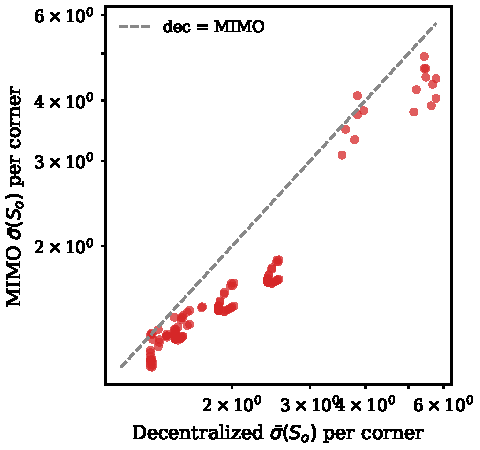
\includegraphics[width=\linewidth]{Figures/fig_corner_scatter.pdf}
    \caption{Per-corner $\bar\sigma(S_o)$, decentralized (horizontal) against MIMO (vertical),
    with the $y=x$ reference line. Points below the line favour the centralized controller: 167
    of 168 in-envelope corners lie there. The out-of-envelope corners --- light load with full
    mismatch, where the share plant gain reaches $K\approx2.07$ --- are the visible cluster in
    which both controllers degrade, the decentralized one slightly more.}
    \label{fig:corner-scatter}
\end{figure}

\subsection{Drive-transient share excursion, in full}

A speed-reference step is applied at $t = \SI{0.05}{\second}$. The small step
($\Delta v_{ref} = +\SI{0.05}{\meter\per\second}$) is fully linear --- zero time on the current
rail --- and is the clean comparison. The large step ($+\SI{2}{\meter\per\second}$) puts the loop
on the $\pm\SI{20}{\ampere}$ rail for $0.18$ to $0.34\,\%$ of the horizon: brief, but enough to
make the comparison partly an anti-windup-recovery comparison and no longer a purely linear one.
The \SI{60}{\second} horizon was chosen so the slow centralized recovery is
measured outright and not reported as a horizon artefact.

\begin{table}[H]
\caption{Drive-transient share excursion. Amplitudes are deviations about
$v_0 = \SI{2}{\meter\per\second}$; horizons are \SI{12}{\second} (small) and \SI{60}{\second}
(large).}
\label{tab:transient}
\begin{tabularx}{\textwidth}{lCCC}
\toprule
\textbf{Quantity} & \texttt{dec} & \texttt{dec500} & \texttt{mimo} \\
\midrule
\multicolumn{4}{l}{\emph{Small signal, $\Delta v_{ref} = +\SI{0.05}{\meter\per\second}$ (0\,\% rail):}} \\
$\max|\Delta\alpha|$, $\Delta V_0 = +0.4$ & 0.01744 & 0.01868 & \textbf{0.00667} \\
$\max|\Delta\alpha|$, $\Delta V_0 = -0.4$ & \textbf{0.01744} & 0.01868 & 0.01935 \\
$\Delta\alpha$ settle ($<0.002$) [\si{\second}] & 0.189 & 0.189 & \textbf{0.175} ($+$) / 0.235 ($-$) \\
$v$ settle (2\,\%) [\si{\second}] & 0.358 & 0.358 & \textbf{0.199} \\
peak $|i_{cmd}|$ [\si{\ampere}] & 2.071 & 2.071 & \textbf{1.179} \\
MIMO/dec excursion ratio & --- & --- & \textbf{0.383} ($+$) / \textbf{1.109} ($-$) \\
\midrule
\multicolumn{4}{l}{\emph{Large signal, $\Delta v_{ref} = +\SI{2}{\meter\per\second}$ (touches the clamp):}} \\
$\max|\Delta\alpha|$, $\Delta V_0 = +0.4$ & 0.3306 & 0.3334 & \textbf{0.1729} \\
$\max|\Delta\alpha|$, $\Delta V_0 = -0.4$ & \textbf{0.3306} & 0.3334 & 0.6289 \\
$\Delta\alpha$ settle ($<0.002$) [\si{\second}] & 0.599 & 0.601 & \textbf{0.337} ($+$) / 0.461 ($-$) \\
$v$ settle (2\,\%) [\si{\second}] & \textbf{0.501} & 0.501 & 22.45 \\
droop span used, $\Delta V_0 = +0.4$ & 0.431--0.850 & 0.431--0.850 & 0.500--0.850 \\
droop span used, $\Delta V_0 = -0.4$ & 0.150--0.569 & 0.150--0.569 & \textbf{0.386--0.719} \\
rail fraction & 0.00337 & 0.00337 & \textbf{0.00187} \\
\bottomrule
\end{tabularx}
\end{table}

\subsection{Regen event on the truth model}

The regen event is run against the 15-state truth model with a bus-voltage output in place of the
8-state design plant. $\Delta v_{ref}$ is stepped to $-\SI{2}{\meter\per\second}$
(\SI{2}{\meter\per\second} to standstill) and $i_{cmd}$ touches the $-\SI{20}{\ampere}$ rail for
$0.18$--$0.34\,\%$ of the horizon; the
\SI{0.8}{\milli\second} prefilter is applied digitally at the base rate since the truth model
carries no $\tau_f$ by convention. Horizon \SI{60}{\second}.

\begin{table}[H]
\caption{Regen event, 15-state truth model. The residual $\Delta v_{bus}$ of \SI{0.105}{\volt} is
the new steady-state load operating point (the vehicle has stopped) and is no tracking error;
recovery is therefore measured about the final value.}
\label{tab:regen}
\begin{tabularx}{\textwidth}{lCCC}
\toprule
\textbf{Quantity} & \texttt{dec} & \texttt{dec500} & \texttt{mimo} \\
\midrule
$\max|\Delta v_{bus}|$ [\si{\volt}] & 1.49112 & 1.49112 & \textbf{1.47429} \\
$\Delta v_{bus}$ final [\si{\volt}] & 0.10478 & 0.10478 & 0.10477 \\
$v_{bus}$ recovery [\si{\second}] & 0.582 & 0.582 & \textbf{0.431} \\
$\max|\Delta\alpha|$ & 0.17467 & 0.17263 & \textbf{0.14478} \\
peak $i_{cmd}$ [\si{\ampere}] & $-20.00$ & $-20.00$ & $-20.00$ \\
rail fraction & 0.00337 & 0.00337 & \textbf{0.00183} \\
$v$ settle (2\,\%) [\si{\second}] & \textbf{0.501} & 0.501 & 22.45 \\
\bottomrule
\end{tabularx}
\end{table}

\begin{figure}[H]
    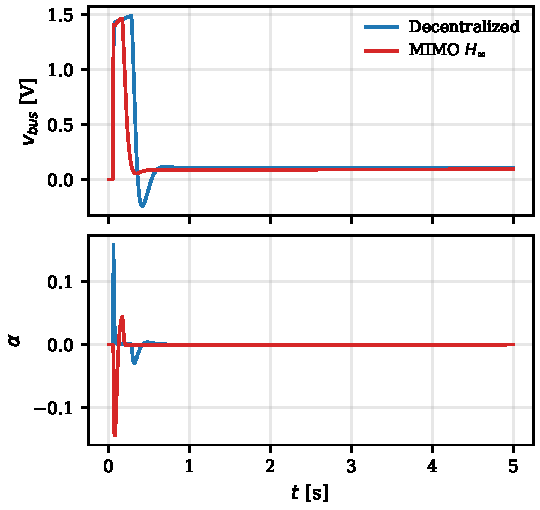
\includegraphics[width=\linewidth]{Figures/fig_regen.pdf}
    \caption{Regen event on the 15-state truth model; the first \SI{5}{\second} of the
    \SI{60}{\second} simulation is shown (the response is in steady state for the remainder).
    Top: bus-voltage deviation. Bottom: share deviation. The bus traces are nearly
    indistinguishable, and not because the event is rail-dominated (the clamp is touched for
    well under $1\,\%$ of the evaluation horizon): the excursion is set by the peak braking
    current both controllers reach, which is a property of the demand and of the plant
    alone.}
    \label{fig:regen}
\end{figure}

\subsection{FC-charge cruise and the drive cycle}

At the FC-charge-cruise operating point ($\SI{2}{\ampere}$, $r_0 = 0.85$, static share
$\alpha_0 = 0.8925$) the energy-management strategy parks the droop ratio on its upper clamp so
the fuel cell carries the bus and the battery charges; the share loop has no upward authority
left by construction. A $+\SI{0.5}{\meter\per\second}$ drive step over a \SI{60}{\second} horizon
shows \textbf{no windup interaction for either controller}: both use only the small downward
authority available ($r_{min} = 0.83693$ and $0.84776$), both converge to a $\sim\SI{2e-3}{}$
residual share error --- a direct consequence of the authority loss, with no sign of a hang --- and neither shows a limit cycle
(tail peak-to-peak $\le 10^{-10}$). All three anti-windup schemes behave gracefully in the
degenerate-authority regime. The two do differ in how long they spend pinned: the decentralized
pair holds the upper clamp for $99.6\,\%$ of the horizon against $0.4\,\%$ for the centralized
controller, and the centralized peak share excursion is correspondingly smaller
(\num{0.06129} against \num{0.10310}, $-41\,\%$). Since the regime is defined by \emph{having no
upward authority}, that difference is a statement about how quickly each controller gives up on
demanding it, and says nothing about disturbance rejection.

The \SI{30}{\second} drive-cycle profile (standstill; ramp 0 to \SI{2}{\meter\per\second} over
\SI{5}{\second}; cruise; coast to \SI{0.5}{\meter\per\second}; hold; stop) with a
$\Delta\alpha_{ref} = +0.2$ share step over 11--\SI{15}{\second} and a $-\SI{1.0}{\ampere}$ load
disturbance over 22--\SI{25}{\second} is where the decentralized advantage is largest: the
whole-cycle RMS speed error is \SI{0.1059}{\meter\per\second} against
\SI{0.2396}{\meter\per\second}, a factor of \num{2.3}, and the RMS share error \num{0.00475}
against \num{0.00730}. The \emph{cruise window} shows why: the decentralized pair is at numerical
zero there ($\SI{2.94e-7}{\meter\per\second}$ RMS speed error) while the centralized controller is
at \SI{0.195}{\meter\per\second}, still recovering from the ramp. On the isolated load disturbance
the decentralized pair is also better by $2.2\times$ in speed
(\SI{0.0191}{} against \SI{0.0420}{\meter\per\second}) though nearly equal in share
(\num{0.0091} against \num{0.0097}). The centralized controller drives
the droop ratio to its \emph{lower} clamp ($r = 0.15$) during the cycle, whereas the decentralized
pair never goes below \num{0.29} --- the cross-channel term spending droop authority in response
to a saturated drive channel, a real cost of centralization on this plant.

\begin{figure}[H]
    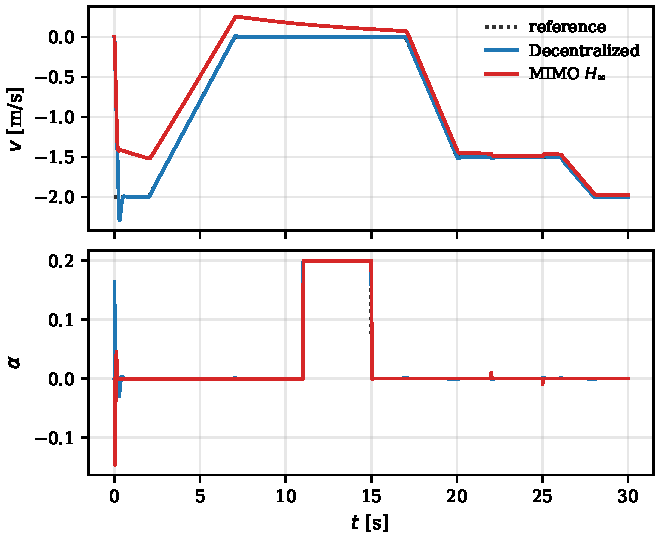
\includegraphics[width=\linewidth]{Figures/fig_drive_cycle.pdf}
    \caption{\SI{30}{\second} drive cycle. Top: speed against reference. Bottom: share against
    reference. The cruise segment (8--\SI{11}{\second}) is where the gap is widest: the
    decentralized pair has settled while the centralized one is still recovering from the ramp.}
    \label{fig:drive-cycle}
\end{figure}

\subsection{Caveats in full}

\begin{enumerate}
\item \textbf{$\Delta V_0$ sign uncertainty bounds any feedforward benefit.} The entire
      centralized coupling advantage lives in \eqref{eq:dalpha}, which is zero at
      $\Delta V_0 = 0$ and flips sign with it. Until $\Delta V_0$ is measured, the defensible
      claim is that the centralized design improves coupling rejection at the design sign and
      degrades it at the mirrored sign.
\item \textbf{The $K$-out-of-envelope corners are waived, and both controllers degrade badly
      there} --- $\bar\sigma(S_o) = 5.77$ decentralized against $4.93$ centralized. The
      stability-only waiver is physically
      justified: these are the 16 light-load, full-mismatch corners where $K\approx2.1$ and the
      static share sits within $\sim0.02$ of the unidirectional-switch feasibility boundary, so
      the plant model itself is at the edge of validity. Neither absolute figure should be read
      as a performance claim.
\item \textbf{Large steps touch the clamp.} The \SI{2}{\meter\per\second} step and the
      drive-cycle ramps reach the $\pm\SI{20}{\ampere}$ clamp for a fraction of a percent of the
      horizon; those comparisons are therefore partly about anti-windup recovery rather than
      about linear design alone.
\item \textbf{The Tier-2 worst-corner numbers come from a representative corner set}: the relative
      verdict survives, the absolute value does not.
\item \textbf{Nothing here is bench-calibrated.} Every calibration item remains open ---
      $\Delta V_0$ above all, plus $k_t$, the encoder chain, $m_{\!e\!f\!f}$, $\tau_v$ and
      $T_{d,v}$. The corner families are wide precisely because of this, but a calibrated plant
      could move the verdicts, particularly the second primary metric.
\end{enumerate}

%---------------------------------------------------------------
\section{MATLAB Cross-Validation}
\label{app:matlab}

The entire chain was cross-checked in MATLAB (Control System and Robust Control Toolboxes) by a
script that independently rebuilds the plant from the documented equations, re-runs
\texttt{hinfsyn} and the MIMO Youla-H correction, parses the emitted coefficient header, and
re-runs the corner battery and the transients. \textbf{The verdict is PASS on all six criteria}
(Table~\ref{tab:matlab}).

\subsection{Scope of the run}
The cross-check was run against the shipped design, at the $\pm\SI{20}{\ampere}$ actuator span
($D_u = \mathrm{diag}(0.35, 20.0)$) used throughout this report, so Table~\ref{tab:matlab}
validates the report as it stands --- plant, synthesis, $T(0)=I$ correction, emitted
coefficient header, corner battery and transients alike. An earlier cross-check at a
$\pm\SI{5}{\ampere}$ span validated the same machinery and algebra at the previous actuator
limit and first identified the two methodological findings recorded below (the
representative-subsample bound on the Tier-2 worst corner, and the distinction between the
continuous and the implemented cross-transfer); the $\pm\SI{20}{\ampere}$ run reconfirms both.
Its numbers are superseded by those in Table~\ref{tab:matlab} and are retained only in the
design record \citep{internal:mimo-cmp}.

\begin{table}[H]
\caption{MATLAB cross-validation anchors for the shipped $\pm\SI{20}{\ampere}$ design. The
right-hand column is the corresponding Python result. The two tools solve the same problem by
independent implementations, so exact agreement is expected only where the quantity is
algebraic; where it is recomputed (the $\gamma$ bisection, a ZOH-discretized sensitivity peak)
the acceptance criterion is stated with the row.}
\label{tab:matlab}
\begin{tabularx}{\textwidth}{XCC}
\toprule
\textbf{Anchor} & \textbf{MATLAB} & \textbf{Python} \\
\midrule
design-plant DC gain (max abs.\ deviation) & \multicolumn{2}{c}{$\SI{2.23e-9}{}$} \\
\texttt{hinfsyn} $\gamma$ & 1.0851 & 0.8977 (bisection) / 1.6456 (a-posteriori) \\
$\|M_{YH} - I\|_2$ & $\SI{9.631e-5}{}$ & $\SI{1.75e-4}{}$ \\
$\mathrm{cond}(G_s(0)Y_H(0))$ & 1.0000 & 1.0001 \\
$T(0)$, in synthesis and on the parsed header & \multicolumn{2}{c}{$I$ exactly} \\
a-posteriori $\|T_{zw}\|_\infty$ of the emitted artefact & 1.6457 & 1.6456 (0.006\,\%) \\
nominal $\bar\sigma(S_o)$ & 1.2623 & 1.2287 (2.7\,\%, criterion $5\,\%$) \\
$\|T_{\alpha\leftarrow v_{ref}}\|_\infty$, implemented \SI{2}{\milli\second} loop & $\SI{1.109e-2}{}$ & $\SI{1.109e-2}{}$ \\
corner battery & \multicolumn{2}{c}{576 / 576 stable} \\
exhaustive-sweep worst $\bar\sigma(S_o)$ & 1.9443 & 1.9445 \\
share excursion, $\Delta V_0 = +0.4 / -0.4$ & 0.00636 / 0.01900 & 0.00667 / 0.01935 \\
peak $|i_{cmd}|$ [\si{\ampere}], $\Delta V_0 = +0.4 / -0.4$ & 1.179 / 1.176 & 1.179 / 1.176 \\
\bottomrule
\end{tabularx}
\end{table}

The \texttt{hinfsyn} level of \num{1.0851} lands between the
Python Riccati bisection (\num{0.8977}) and the a-posteriori achieved level (\num{1.6456}),
which is precisely the behaviour the $P_f$ degeneracy of Appendix~\ref{app:dgkf} predicts: the
bisection is optimistic because its feasibility test is vacuous, and a third implementation
therefore has no reason to reproduce either endpoint. The two values of $\|M_{YH}-I\|_2$
($\SI{9.6e-5}{}$ and $\SI{1.75e-4}{}$) are computed on separately synthesized controllers and
are quoted as computed; both say the same thing, that the $H_\infty$ controller was already
integral to four decimals. And the nominal $\bar\sigma(S_o)$ differs by $2.7\,\%$ because
MATLAB evaluates the ZOH-discretized loop where the Python figure is continuous; the criterion
for that row is $5\,\%$.

\begin{figure}[H]
    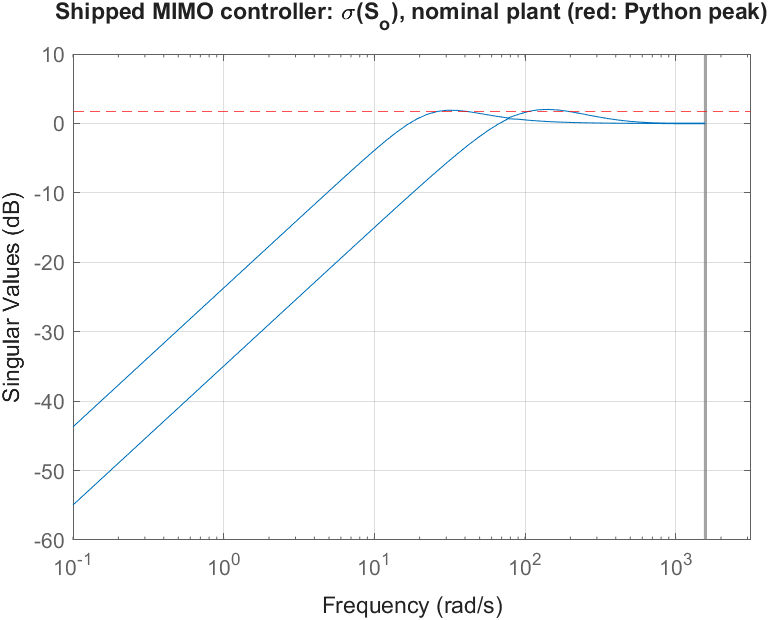
\includegraphics[width=\linewidth]{Figures/MATLAB_mimo_sigmaS.png}
    \caption{MATLAB cross-check of $\bar\sigma(S_o)$ versus frequency, built independently from
    the documented plant equations and the parsed coefficient header, for the shipped
    $\pm\SI{20}{\ampere}$ design. Compare Figure~\ref{fig:sigma-S-both}: the shapes and the
    peak levels agree, the residual difference being that this curve is evaluated on the
    ZOH-discretized loop.}
    \label{fig:matlab-sigma}
\end{figure}

\begin{figure}[H]
    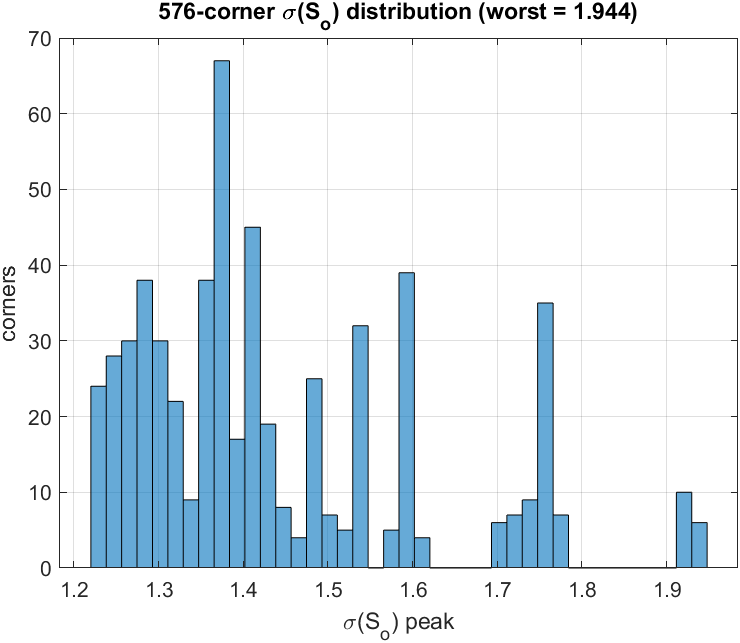
\includegraphics[width=\linewidth]{Figures/MATLAB_mimo_corner_scatter.png}
    \caption{MATLAB cross-check of the per-corner robustness scatter (compare
    Figure~\ref{fig:corner-scatter}), for the shipped $\pm\SI{20}{\ampere}$ design. This sweep
    is the \emph{full} $24\times24$ family at the nominal operating point, where
    Figure~\ref{fig:corner-scatter} is the representative subsample; it is what establishes
    that the subsample misses worse corners.}
    \label{fig:matlab-scatter}
\end{figure}

Two methodological findings were first surfaced by the $\pm\SI{5}{\ampere}$ run and are
reconfirmed here, so both are structural and no artefact of a
particular actuator span. First, the MATLAB sweep is exhaustive at the nominal operating point,
and it locates the worst $\bar\sigma(S_o)$ corner \emph{outside} the Python representative
corner set: $\bar\sigma(S_o) = \num{1.9443}$ at $\Delta V_0 = -0.4$,
$T_d = \SI{2}{\milli\second}$, $\tau_r = \SI{300}{\micro\second}$,
$\tau_f = \SI{0.8}{\milli\second}$, $K_v = 2$, damping factor 2,
$\tau_v = \SI{5}{\milli\second}$, $T_{d,v} = \SI{4}{\milli\second}$, against the
representative-set figure of \num{1.8754} reported in Table~\ref{tab:sigma}. The Python model
reproduces that corner independently at \num{1.9445}, and stability is unaffected (576/576
here, 0/4992 on Tier-1). That is why the Tier-2 worst-corner figure is reported throughout as a
subsample lower bound rather than as a certificate. Second, the nominal cross-transfer
improvement is a \emph{continuous-domain} figure and must be requoted on the implemented
\SI{2}{\milli\second} loop; MATLAB obtains $\SI{1.109e-2}{}$ there, matching the implemented-loop
row of Table~\ref{tab:sigma} exactly, which is why that table carries both rows. The two
implementations agree everywhere they should agree, and the residual differences are
attributable to the stated approximations alone.

\subsection{Reproduction tolerance}
The share-channel controller is re-derived here from its documented weights instead of parsed
from the firmware header, and the re-derivation carries a $0.67\,\%$ integrator-gain offset
(112.679 against 111.930) attributable to solver accuracy at the $\gamma_{opt}$ anchor. The offset
is well inside the corner family and affects no comparison in this report.

%---------------------------------------------------------------
\section{Anti-Windup and Discretization}
\label{app:aw}

For the standard configuration
$\hat u/\hat n = -Y$ (\citep{assadian2020neoclassical} \S3.8.2, eq.~(3.124), p.~132): the
Youla transfer function \emph{is} the noise-to-actuator map. The $W_u$ weight acting on $Y$ in
Table~\ref{tab:mimo-weights} is therefore a direct bound on actuator activity, and the anti-windup
schemes below handle the residual demand that the weight does not remove.

\subsection{Decentralized baseline: Hanus self-conditioning}

The SISO drive controller's \emph{non-integral} branch alone has a DC gain of
\SI{367.7}{\ampere\per\meter\per\second}, so it saturates the $\pm\SI{20}{\ampere}$ actuator for
speed errors above $e_{sat} = \SI{54.4}{\milli\meter\per\second}$ and its lag states wind up
independently of the integrator. The threshold scales with the clamp, so the scheme's adequacy is
an amplitude question: integrator-only back-calculation is clean on steps up to
\SI{0.2}{\meter\per\second} (final errors of order $\SI{e-8}{\meter\per\second}$, no limit cycle)
and fails from \SI{0.5}{\meter\per\second}, producing a \SI{-0.101}{\meter\per\second} standing
error and a \SI{6.3}{\milli\meter\per\second} limit cycle on the 0 to \SI{2}{\meter\per\second}
step. Because that step is a required gate, the baseline uses Hanus
self-conditioning \citep{hanus1987conditioning} on a five-state state-space realization,
$x_{k+1} = (A_d - B_d C_d/D_d)x_k + B_d u/D_d$ with $u$ the clamped output --- exactly equivalent
to the biquad-plus-integrator form when unsaturated (verified to $\SI{6.32e-10}{\ampere}$), but
\emph{not} implementable as a biquad cascade. This is the origin of the six implemented states in
Table~\ref{tab:cost}.

\subsection{Centralized controller: reduction, discretization, modal form}

The controller $G_{c,YH}$ has order 30 (14 controller $+$ 8 plant $+$ 8 from the Youla
interconnection); after the integrator split the stable remainder is order 28. Balanced truncation
selects order 7 at a $10^{-2}$ margin, with a maximum relative $\bar\sigma$ deviation of
$\SI{1.88e-3}{}$ over $\omega\in[0.1, 10^4]$ against a $2\times10^{-2}$ tolerance. Deviation is
measured per frequency instead of against a single global scale, which would be dominated by the
integrator's low-frequency magnitude and would make the check vacuous. The final continuous
controller is 9 states: two exact integrators plus a seven-state remainder.

The integrator is an exact $2\times2$ Tustin block with the matrix $K_I$, kept separate from the
remainder so anti-windup can act on it; the recursive trapezoid form is verified equal to the LTI
form at $\SI{2.8e-17}{}$. \emph{Ordering matters}: the integrator is advanced first and the new
value used in the output, matching the firmware idiom --- advancing it afterwards inserts a hidden
extra sample of delay, which the equivalence check catches. The stable remainder is discretized by
Tustin and transformed to real modal (block-diagonal) form,
$A_{modal} = \mathrm{diag}(-0.9866,\,0.9225,\,0.6205,\,
\left[\begin{smallmatrix}-0.8592 & 0.0737\\ -0.0737 & -0.8592\end{smallmatrix}\right],\,
\left[\begin{smallmatrix}-0.0995 & 0.2398\\ -0.2398 & -0.0995\end{smallmatrix}\right])$,
at $\mathrm{cond}(T) = 7.24$ and reproducing the Tustin response to $\SI{7.9e-16}{}$. The
rationale is float32: a modal $A$ has the pole locations themselves as its coefficients, so
rounding perturbs each mode independently instead of perturbing companion-form polynomial
coefficients, where a $10^{-7}$ relative error can move clustered roots by far more.

\subsection{Centralized anti-windup: back-calculation plus authority clamp}

Anti-windup has two parts. Because the integrator state adds directly to the scaled input, its
output map is $I_2$ and the back-calculation map is exactly $D_u^{-1}$: on saturation,
$x_{int} \mathrel{+}= D_u^{-1}\delta$ with $\delta = u_{sat}-u$ physical, and
$\mathrm{cond}(D_u^{-1}) = 57.14$ so no diagonal fallback is needed --- the
directionality-preserving generalization of the scalar scheme. On top of it, $x_{int}$ is clamped
componentwise to $[-1,1]^2$: the integrator alone may never demand more than the actuator can
deliver.

The second term guards against bare back-calculation dumping the \emph{whole} clamp excess into
the integrator, including the part created by the direct feedthrough --- which lets the integrator
absorb a direct-term excess and then hold the \emph{opposite} rail once the error collapses. The
scalar share controller's direct term is small enough for this to be harmless there. Here the
scaled direct term is $D_{22} = 0.111$ against a peak $|K_{22}|$ of \num{1.33}: about $8\,\%$,
non-negligible but no longer the acute driver it was at a four-times-smaller actuator span, where
the same ratio sat on four-times-larger scaled numbers. \textbf{The clamp is retained as
defence-in-depth rather than as a necessity}: it costs two comparisons per tick, it bounds a
failure mode whose severity is a function of the input scaling (and therefore of a number that has
already moved once), and the integrator alone should never be able to demand more than the
actuator can deliver in any case. The mechanism is exposed only by a closed-loop recovery
simulation (rail at $-\SI{20}{\ampere}$, hold, release: \SI{110}{\milli\second} on the rail,
release within one tick, a $\SI{4.0e-4}{\meter\per\second}$ recovery tail, no sustained rail). An
open-loop ``hold a large error then zero it'' test cannot reveal it, because a loop with an
externally pinned error has no mechanism to unwind.

At this actuator span the \SI{0.5}{\meter\per\second} drive step no longer saturates at all --- it
peaks at \SI{11.79}{\ampere} and settles in \SI{150}{\milli\second} to \num{0.500000} --- so the
closed-loop recovery simulation above is the only place the $T(0)=I$ property is exercised
\emph{through} a saturation episode. It survives it unbiased. The slow tail seen on larger steps
is governed by $K_{I,22} = 0.103$ against a \SI{0.122}{\radian\per\second} plant pole and is loop
shaping, \emph{not} a windup hang.

%=====================================
% References — embedded thebibliography (project convention; no .bib pipeline)
%=====================================
\begin{adjustwidth}{-\extralength}{0cm}

\reftitle{References}

\begin{thebibliography}{99}

\bibitem{zhou1996robust}
Zhou, K.; Doyle, J.C.; Glover, K. \textit{Robust and Optimal Control}; Prentice Hall: Upper
Saddle River, NJ, USA, 1996.

\bibitem{skogestad2005multivariable}
Skogestad, S.; Postlethwaite, I. \textit{Multivariable Feedback Control: Analysis and Design},
2nd ed.; Wiley: Chichester, UK, 2005.

\bibitem{assadian2020neoclassical}
Assadian, F.; Mallon, K. \textit{Neoclassical Control: Control Systems and Estimation Design
Using the Youla Parameterization Technique}; draft manuscript, John Wiley \& Sons: Hoboken, NJ,
USA, dated 13 October 2020.
% TODO(verify): all section, equation and page numbers in this report cite the 2020 draft
% manuscript (the version consulted). Re-check every one against the published 2022 edition
% (\bibitem{assadian2022robust}) before any circulation wider than the lab.

\bibitem{assadian2022robust}
Assadian, F.; Mallon, K.R. \textit{Robust Control: Youla Parameterization Approach};
John Wiley \& Sons: Hoboken, NJ, USA, 2022.

\bibitem{tan2025scaling}
Tan, R.; Yadav, S.; Assadian, F. Systemic scaling of powertrain models with Youla and
$\mathcal{H}_\infty$ driver control. \textit{Energies} \textbf{2025}, \textit{18}, 3126.
\url{https://doi.org/10.3390/en18123126}

\bibitem{tan2025youlah}
Tan, R.; Yadav, S.; Assadian, F. A Practical Youla Gain-Tuning Framework for $H_\infty$
Controller Realization. Manuscript in preparation, 2026.
% TODO(verify): confirm final venue/status before citing externally.

\bibitem{hanus1987conditioning}
Hanus, R.; Kinnaert, M.; Henrotte, J.-L. Conditioning technique, a general anti-windup and
bumpless transfer method. \textit{Automatica} \textbf{1987}, \textit{23}, 729--739.
% TODO(verify): page range checked against the standard citation, not the original article.

\bibitem{doyle1989state}
Doyle, J.C.; Glover, K.; Khargonekar, P.P.; Francis, B.A. State-space solutions to standard
$H_2$ and $H_\infty$ control problems. \textit{IEEE Trans. Autom. Control} \textbf{1989},
\textit{34}, 831--847.

\bibitem{internal:droop}
Tan, R. Robust Power Sharing Control in a Hybrid Energy System Using Droop Control. Manuscript
in preparation, 2026. Internal reference: \texttt{papers/Droop\_Control/}, with design record
\texttt{controller\_design/system\_model.md} and
\texttt{controller\_design/controller\_synthesis.md}.

\bibitem{internal:mimo-model}
Tan, R. MIMO Share/Drive Plant Model. Internal design record,
\texttt{controller\_design\_MIMO/mimo\_system\_model.md}, 2026.

\bibitem{internal:mimo-synth}
Tan, R. Centralized $2\times2$ MIMO $H_\infty$ / Youla-H Controller --- Design Record. Internal
design record, \texttt{controller\_design\_MIMO/}\allowbreak\texttt{mimo\_synthesis.md}, 2026.

\bibitem{internal:mimo-cmp}
Tan, R. MIMO vs.\ Decentralized --- Comparison Results. Internal design record,
\texttt{controller\_design\_MIMO/mimo\_comparison.md}, 2026.

\end{thebibliography}

\PublishersNote{}
\end{adjustwidth}
\end{document}
